\documentclass[11pt]{article}
\usepackage[margin=1in]{geometry}

\usepackage{amsmath}
\usepackage{amssymb}
\usepackage{amsfonts}
\usepackage{amsthm}
\usepackage{thm-restate}
\usepackage{subcaption}
\usepackage{cleveref}
\usepackage[utf8]{inputenc}
\usepackage{makecell}
\usepackage[dvipsnames]{xcolor}
\usepackage{tcolorbox}
\usepackage{enumerate}
\usepackage{tikz}
\newcommand{\pathonecolor}{Blue!40}
\newcommand{\pathtwocolor}{Red!60}
\newcommand{\paththreecolor}{Yellow!60}
\newcommand{\pathfourcolor}{Brown!50}
\newcommand{\pathfivecolor}{Purple!60}
\newcommand{\pathsixcolor}{ForestGreen!80}

\newtheorem{theorem}{Theorem}
\newtheorem{lemma}{Lemma}

% tikz stuff
\tikzset{every picture/.append style={semithick, >=stealth}}
\tikzset{every node/.style={circle, inner sep = 2pt}}
\pgfdeclarelayer{background}
\pgfsetlayers{background,main}
\usetikzlibrary{decorations.pathreplacing, fit}

\newcommand{\alexcom}[1]{\textcolor{brown}{(Alex: #1)}}
\newcommand{\arielcom}[1]{\textcolor{teal}{(Ariel: #1)}}
\newcommand{\andicom}[1]{\textcolor{orange}{(Andi: #1)}}


\newcommand{\paths}{\mathcal{P}}
\newcommand{\antichains}{\mathcal{A}}
\newcommand{\chains}{\mathcal{C}}
\newcommand{\ints}{\mathbb{Z}}
\newcommand{\sets}{\mathcal{S}}

\bibliographystyle{plainurl}% the mandatory bibstyle

\title{Maximum Coverage $k$-Antichains and Chains: A Greedy Approach\thanks{This work has received funding from the European Research Council (ERC) under the European Union's Horizon 2020 research and innovation programme (grant agreement No.~851093, SAFEBIO), and from the Research Council of Finland grants No.~346968, 358744. Manuel Cáceres is supported by the Helsinki Institute for Information Technology.}} %TODO Please add

%\titlerunning{Dummy short title} %TODO optional, please use if title is longer than one line

\author{Manuel Cáceres\thanks{Department of Computer Science, Aalto University, Finland, \texttt{manuel.caceres@aalto.fi}.}
\and Andreas Grigorjew\thanks{University of Helsinki, Finland, \texttt{andreas.grigorjew@helsinki.fi}.}
\and Wanchote Po Jiamjitrak\thanks{University of Helsinki, Finland, \texttt{wanchote.jiamjitrak@helsinki.fi}.}
\and Alexandru I. Tomescu\thanks{University of Helsinki, Finland, \texttt{alexandru.tomescu@helsinki.fi}.}}



\begin{document}

\date{}

\maketitle


\begin{abstract}
Given an input acyclic digraph $G = (V,E)$ and a positive integer $k$, the problem of Maximum Coverage $k$-Antichains (resp., Chains) denoted as MA-$k$ (resp., MC-$k$) asks to find $k$ sets of pairwise unreachable vertices, known as antichains (resp., $k$ subsequences of paths, known as chains), maximizing the number of vertices covered by these antichains (resp. chains). While MC-$k$ has been recently solved in (almost) optimal $O(|E|^{1+o(1)})$ time~[Kogan and Parter, ICALP 2022], the fastest known algorithm for MA-$k$ is a recent $(k|E|)^{1+o(1)}$-time solution~[Kogan and Parter, ESA 2024] as well as a $1/2$ approximation running in $|E|^{1+o(1)}$ time in the same paper.

In this paper, we leverage a paths-based proof of the Greene-Kleitman (GK) theorem with the help of the greedy algorithm for set cover and recent advances on fast algorithms for flows and shortest paths to obtain the following results for MA-$k$:
\begin{itemize}
    \item The first (exact) algorithm running in $|E|^{1+o(1)}$ time, hence independent in $k$.
    \item A randomized algorithm running in $\tilde{O}(\alpha_k 
    |E|)$ time\footnote{Our $\tilde{O}$ notation hides polylog factors.}, where $\alpha_k$ is the size of the optimal solution. That is, a near-linear parameterized running time, generalizing the result of~[Mäkinen et al., ACM TALG] obtained for $k=1$.
    \item An approximation algorithm running in time $O(\alpha_1^2|V| + (\alpha_1+k)|E|)$ with approximation ratio of $(1-1/e) > 0.63 > 1/2$.
\end{itemize}
Our last two solutions rely on the use of \texttt{greedy} set cover, first exploited in~[Felsner et al., Order 2003] for chains, which we now apply to antichains. We complement these results with two examples (one for chains and one for antichains) showing that, for every $k \ge 2$, \texttt{greedy} misses a $1/4$ portion of the optimal coverage. We also show that \texttt{greedy} is a $\Omega(\log{|V|})$ factor away from minimality when required to cover all vertices: previously unknown for sets of chains or antichains.

Finally, some of our intermediate results show efficient solutions to related problems, which can be of independent interest.
\end{abstract}

\section{Introduction}

For a directed acyclic graph (DAG) $G = (V, E)$, a chain is a subsequence of the vertices of a path (equivalently a path in the transitive closure of $G$, $TC(G)$) and an antichain is a set of vertices that are pairwise unreachable (equivalently, an independent set in $TC(G)$). The problem of Maximum Coverage $k$-antichains (MA-$k$) asks to find a set of $k$ pairwise disjoint antichains whose union size is maximized: we say that one such optimal solution \emph{covers} the $\alpha_k$ vertices in this union. The problem of Maximum Coverage $k$-chains (MC-$k$) is analogously defined and one such optimal solution covers $\beta_k$ vertices.

Strongly related to these coverage problems are the minimum partition problems: find the minimum number of pairwise disjoint antichains (analogously chains) partitioning the vertices of $G$, MAP (resp. MCP). Mirsky~\cite{mirsky1971dual} and Dilworth~\cite{dilworth1987decomposition} were the first to draw a connection between the maximum coverage and minimum partition problems. On the one hand, Mirsky proved that the number of antichains in a MAP equals $\beta_1$, also known as the \emph{height} of $G$. On the other hand, Dilworth proved that the number of chains in a MCP equals $\alpha_1$, also known as the \emph{width} of $G$. Later, Greene and Kleitman~\cite{greene1976structure,greene1976some} completed this connection with the celebrated Greene-Kleitman (GK) theorems\footnote{The generalization of Mirsky's results is due to Greene only~\cite{greene1976some}, we use GK to refer to both theorems for simplicity.}: $\alpha_k$ (resp. $\beta_k$) is equal to the minimum \emph{$k$-norm} of a chain (resp. antichain) partition\footnote{We provide a formal definition of $k$-norm in \Cref{sec:preliminaries}.}. We denote partitions with minimum $k$-norm by MCP-$k$ and MAP-$k$, respectively.


From an algorithmic perspective, on the one hand, it is a well-known result that we can solve MAP and MC-$1$ in linear time: by a simple DP one can compute the length of the longest path ending at each vertex (solving MC-$1$), moreover a partition of the vertices according to these lengths gives a MAP. On the other hand, Fulkerson~\cite{fulkerson1956note} was the first to show a polynomial-time algorithm for MCP and MA-$1$ by reducing the problem to maximum bipartite matching. However, Fulkerson's algorithm computes a maximum matching over $TC(G)$. Modern solutions avoid working directly on $TC(G)$ since its size can be quadratic in $G$. The state-of-the-art solutions are the almost linear $|E|^{1+o(1)}$-time solution of Cáceres~\cite{caceres2023minimum}, the (parameterized linear) $O(\alpha_1^2|V|+|E|)$-time algorithm of Cáceres et~al.~\cite{caceres2022sparsifying,caceres2022minimum} and the (parameterized near-linear) $\tilde{O}(\alpha_1|E|)$-time solution of Mäkinen et~al.~\cite{makinen2019sparse}. The latter algorithm by Mäkinen et~al.~\cite{makinen2019sparse} computes a \texttt{greedy} chain partition, which is then shrunk to minimum size. In fact, this \texttt{greedy} solution is exactly the output of the well-known \texttt{greedy} set cover~\cite{chvatal1979greedy} with sets corresponding to the chains of the DAG. This idea was originally proposed by Felsner et~al.~\cite{felsner2003recognition} for transitive DAGs, and it was later optimized for general DAGs~\cite{kowaluk2008path,makinen2019sparse}, avoiding the computation of $TC(G)$. Although, the \texttt{greedy} chain partition inherits the $O(\log{n})$ approximation ratio from \texttt{greedy} set cover, it is still unknown whether it is tight for chains in DAGs.

In the case of the coverage problems, MC-$k$~\cite{kogan2022beating,caceres2023minimum} has been solved in (almost) optimal $|E|^{1+o(1)}$ time via a reduction to Minimum Cost Flow. However, until recently, the fastest solution for MA-$k$ was an $O(|V|^3)$-time algorithm from the 80's~\cite{gavril1987algorithms}. The big difference in the running times between both problems was tantalizing and Kogan and Parter~\cite{kogan2024algorithmic} tackled this gap by exploiting algorithmic properties of the GK theorems. They present an elegant $1/2$ approximation running in time $|E|^{1+o(1)}$, as well as an approximation scheme (only for transitive DAGs) running in time $O(\alpha_k\sqrt{|E|}|V|^{o(1)}/\epsilon + |V|)$. The same paper also shows an exact solution running in $(k|E|)^{1+o(1)}$ time beating the $O(|V|^3)$-time algorithm of Gavril.

\subsection{Overview of Our Results}

The initial proof of the GK theorems by Greene and Kleitman~\cite{greene1976structure,greene1976some} was based on lattice theoretic methods, with little algorithmic insight. Saks~\cite{saks1979short} presented an elegant combinatorial proof by using the product between a poset and a chain of length $k$, which is exploited in the state-of-the-art $(k|E|)^{1+o(1)}$-time solution~\cite{kogan2024algorithmic}. Later, Frank~\cite{frank1980chain} presented an algorithmic proof based on a reduction to minimum cost flow on the same graph used on Fulkerson's proof~\cite{fulkerson1956note}. As such, the corresponding algorithm runs on $TC(G)$, making it too slow. However, this proof also shows the existence of orthogonal optimal solutions for ranging values of $k$, which is exploited in the state-of-the-art $|E|^{1+o(1)}$-time $1/2$ approximation~\cite{kogan2024algorithmic}. 

In this paper we leverage a less known algorithmic proof of the GK theorems found in Schrijver's book~\cite[Theorem 14.8 \& Theorem 14.10]{schrijver2003combinatorial}. These proofs are also based on reductions to minimum cost flow which work directly on $G$, avoiding the computation of $TC(G)$. Our main contribution is adapting Schrijver's proofs and showing that the problems can be solved by a constant number of minimum cost flow reductions. We use the recent results on minimum cost flow~\cite{chen2022maximum,van2023deterministic} to obtain our first results.

\begin{restatable}{theorem}{almostlinearalgo}\label{thm:almostLinear}
    Given a DAG $G = (V, E)$ and a positive integer $k$, we can solve the problems MCP-$k$, MA-$k$, MC-$k$ and MAP-$k$ in almost optimal $O(|E|^{1+o(1)})$ time.
\end{restatable}

We note that in~\cite{kogan2024algorithmic} it was shown how to compute MCP-$k$~\cite[Lemma 4.4]{kogan2024algorithmic}, MP-$k$ and MC-$k$~\cite[Lemma 4.6]{kogan2024algorithmic} by a logarithmic number of minimum cost flow computations. Our result is stronger in the sense that only one minimum cost flow is required, and we additionally solve MA-$k$ in almost optimal time, previously unknown.

Although \Cref{thm:almostLinear} solves the problems up to subpolynomial factors, it is still relevant to investigate whether faster and/or simpler solutions can be achieved by the means of parameterization. As mentioned earlier, two state-of-the-art solutions for $k=1$ (MCP and MA-$1$) run in time $O(\alpha_1^2|V|+|E|)$~\cite{caceres2022sparsifying,caceres2022minimum} and $\tilde{O}(\alpha_1|E|)$~\cite{makinen2019sparse}, which is linear and near-linear for constant values of $\alpha_1$, respectively. It is natural to ask whether such results can be obtained for general $k$. We obtain the following result.

\begin{restatable}{theorem}{nearlinearalgo}\label{thm:nearLinear}
    Given a DAG $G = (V, E)$ and a positive integer $k$, we can solve the problems MCP-$k$ and MA-$k$ in parameterized near optimal $\tilde{O}(\alpha_k|E|)$ time and the problems MAP-$k$ and MC-$k$ in parameterized near optimal $\tilde{O}(\beta_k|E|)$ time. Algorithms are randomized Las Vegas and running times are with high probability (and in expectation).
\end{restatable}

To achieve this, we combine the recent results for negative cost cycles~\cite{bernstein2022negative,bringmann2023negative} with the simple cycle-canceling method. In fact, the minimum cost flow values in Schrijver's reductions are $\alpha_k-|V|$ and $-\beta_k$, respectively. This simple observation directly derives the result for $\beta_k$. To derive the result for $\alpha_k$, we devise an initial solution based on \texttt{greedy} for weighted set cover and prove that the cost of such solution is $\tilde{O}(\alpha_k)$ away from the optimal. As such, this can be seen as a generalization of the results in~\cite{makinen2019sparse} for $k>1$. 

Our last algorithmic results are approximation algorithms based on \texttt{greedy} set cover and are independent of Schrijver's reductions. In more detail, it follows from bounds on set cover~\cite{hochbaum1996approximating} that the first $k$ \texttt{greedy} chains and antichains cover at least a $(1-1/e)$ fraction of $\beta_k$ and $\alpha_k$, respectively, beating the state-of-the-art $1/2$ approximation~\cite{kogan2024algorithmic}. Our main contribution is to apply \texttt{greedy} to the set of antichains, and to show how these antichains can be computed efficiently.

\begin{restatable}{theorem}{approxalgo}\label{thm:approxAlgo}
    Given a DAG $G = (V, E)$ and a positive integer $k$, there exist $(1-1/e)$-approximation algorithms solving MC-$k$ in $O(k|E|)$ time and MA-$k$ in $O(\alpha_1^2|V|+ (\alpha_1+k)|E|)$ time.
\end{restatable}


We note that the result for MC-$k$ is a direct consequence of the algorithm of Mäkinen et~al.~\cite{makinen2019sparse}. For MA-$k$ we show how to compute $k$ \texttt{greedy} antichains in $O((\alpha_1+k)|E|)$ time after using the algorithm of Cáceres et~al.~\cite{caceres2022sparsifying,caceres2022minimum}. Our solution relies on the duality between MCP and MA-$1$ over a subset of vertices, and uses this duality to amortize the computation of the $k$ \texttt{greedy} antichains.


We complement our algorithmic contributions with the first (to the best of our knowledge) study of the limitations of \texttt{greedy} applied to sets of chains or sets of antichains, as previously exploited in the literature and in this paper. As previously stated, \texttt{greedy} inherits the bounds of set cover. Namely, it is a $\ln{n}$ approximation for the partition problems~\cite{chvatal1979greedy} and a $(1-1/e)$ approximation for the coverage problems~\cite{hochbaum1996approximating}. It is known that these bound are tight for general set systems~\cite{slavik1996tight,feige1998threshold}, however, it remains unknown whether these bounds are tight for sets of chains or antichains of a DAG. We show the following.

\begin{restatable}{theorem}{upperboundcoverage}\label{thm:upperBoundCoverage}
    For every $k\ge 2$, there exists a DAG, such that $k$ \texttt{greedy} chains cover only $3/4$ of $\beta_k$. The same result holds for $k$ \texttt{greedy} antichains and $\alpha_k$.
\end{restatable}

We obtain this result by creating tight DAG instances where \texttt{greedy} covers exactly a $(1-(1-1/k)^k)$ fraction of the optimal, for $k=2,3$. Generalizing these results for $k>3$ would prove the same $(1-1/e)$ ratio as for general set systems. For the partition problems we obtain the following result.


\begin{restatable}{theorem}{lowerboundpartition}\label{thm:lowerBoundPartition}
    For MCP, there exists a class of DAGs of increasing size, such that the number of chains taken by \texttt{greedy} is a $\log_4(|V|)$ factor away from the optimal $\alpha_1=2$. For MAP, the same result holds for \texttt{greedy} antichains and $\beta_1=2$.
\end{restatable}

Although these results do not match the upper bound of $\ln{n}$, they are the first to demonstrate the approximation ratio to be $\Omega(\log{n})$. Moreover, since the results hold for constant ($=2$) optimal solution, it also disproves the number of \texttt{greedy} chains or antichains to be a function of the optimal solution, that is, $\alpha_1$ or $\beta_1$, respectively.

See \Cref{tab:acronyms,tab:our-results} in \Cref{appendix:acronyms} for a detailed summary of the state-of-the-art and our algorithmic results. The rest of the paper is organized as follows. In the next section, we present the technical notation used in the paper as well as preliminary results, including Schrijver's reductions. The next sections are dedicated to prove \Cref{thm:almostLinear}, \Cref{thm:nearLinear}, \Cref{thm:approxAlgo} and, \Cref{thm:upperBoundCoverage,thm:lowerBoundPartition}, respectively.


\section{Notation and Preliminaries}\label{sec:preliminaries}

We use $G = (V, E)$ and $k$ to denote our input DAG and a positive integer, respectively. We denote paths $P$ and chains $C$ (subsequences of paths) by their sequence of vertices, but we also use $P$ and $C$ to refer to the corresponding sets of vertices. As such, their \emph{lengths} are $|P|$ and $|C|$, respectively. Antichains are sets of pairwise unreachable vertices denoted by $A$. We use $\paths,\chains$ and $\antichains$ to denote collections of paths, chains and antichains, respectively, and $V(\paths), V(\chains), V(\antichains)$ to denote the corresponding vertices in these collections, e.g. $V(\chains) = \bigcup_{C\in\chains} C$ and $|V(\chains)|$ is the \emph{coverage} of $\chains$. In the collections of chains $\chains$ and antichains $\antichains$ used in this paper, the chains/antichains are pairwise disjoint. However, pairs of paths in collections of paths $\paths$ might intersect. If $v \in A$ (or $P$ or $C$) we say that $A$ \emph{covers} $v$, if additionally $A\in \antichains$ (or $\chains$ or $\paths$) we also say that $\antichains$ covers $v$. If $V = V(\paths)$ we say that $\paths$ is a path \emph{cover}. If $V = V(\chains)$ (resp. $V(\antichains)$) we say that $\chains$ is a chain (resp. antichain) \emph{partition}. The celebrated GK theorems state:

\begin{theorem}[Greene-Kleitman (1976)]\label{thm:GK}
The following two equalities hold:
\begin{align*}
    \alpha_k := \max_{\antichains: |\antichains| = k} |V(\antichains)| &= \min_{\chains:V = V(\chains)}\sum_{C \in \chains} \min(|C|, k)\\
    \beta_k := \max_{\chains: |\chains| = k} |V(\chains)| &= \min_{\antichains:V = V(\antichains)}\sum_{A \in \antichains} \min(|A|, k)
\end{align*}
\end{theorem}


For a chain (or antichain) partition $\chains$, $\sum_{C \in \chains} \min(|C|, k)$ is known as the $k$-norm of $\chains$. In addition to MC-$k$ and MA-$k$, we use MP-$k$ to refer to a collection of $k$ paths covering $\beta_k$ vertices\footnote{Note that any MC-$k$ can be extended to a MP-$k$ and vice versa.}. A path cover of minimum size is denoted MPC. We also use the same notation to refer to the corresponding problems of finding one such optimal collections. See \Cref{tab:acronyms} in \Cref{appendix:acronyms} for a summary of the acronyms we use. Unfortunately, there might be no path cover with $k$-norm exactly $\alpha_k$ (as paths can be forced to cover vertices multiple times, see e.g.~\cite[Figure 1]{caceres2023minimum}). Schrijver~\cite{schrijver2003combinatorial} extended the definition of $k$-norm to collections of paths and (pairwise disjoint) antichains, and proved the following version of the GK theorems.

\begin{restatable}[Schrijver (2003)]{theorem}{GKCollections}\label{thm:GKCollections}
The following two equalities hold:
\begin{align*}
    \alpha_k &= \min_{\paths}|V\setminus V(\paths)| + k|\paths|\\
    \beta_k &= \min_{\antichains}|V\setminus V(\antichains)| + k|\antichains|
\end{align*}
\end{restatable}

Schrijver used a reduction to minimum cost circulation to prove these equalities. As these reductions are central to this work, we show them later in this section. For a collection of paths (resp. antichains) $\paths$, $|V\setminus V(\paths)| + k|\paths|$ is known as the $k$-norm of $\paths$. We use MAS-$k$ (resp. MPS-$k$) to denote a collection of antichains (resp. paths) of minimum $k$-norm. In our proofs we use the following results relating the different collections of chains, antichains and paths.

\begin{lemma}\label{lem:relations}
    Define the \emph{partition completion} of a collection of chains (or antichains) $\chains$ as $\chains^V := \chains \cup \{\{v\} \mid v \in V\setminus V(\chains)\}$. Then, the following statements hold.
    \begin{enumerate}
        \item If $V(\paths) = V(\chains)$, $|\chains| = |\paths|$ and $|C| \ge k$ for all $C \in \chains$, then the $k$-norm of $\paths$ equals the $k$-norm of $\chains^V$.
        \item If $|A| \ge k$ for all $A\in\antichains$, then the $k$-norm of $\antichains$ equals the $k$-norm of $\antichains^V$.
        \item If $\antichains$ is a MAS-$k$, then $\antichains^V$ is a MAP-$k$.
    \end{enumerate}
\end{lemma}
\begin{proof}
    \begin{enumerate}
        \item The $k$-norm of $\chains^V$ is 
        \begin{align*}
            \sum_{C\in\chains^V} \min(|C|,k) &=  \sum_{C\in \{\{v\} \mid v \in V\setminus V(\chains)\}} \min(|C|,k) + \sum_{C\in\chains} \min(|C|,k)\\  
            &= |V\setminus V(\chains)| + k|\chains| \\
            &= |V\setminus V(\paths)| + k|\paths|
        \end{align*}
        And thus equal to the $k$-norm of $\paths$.
        \item The $k$-norm of $\antichains^V$ is
        \begin{align*}
            \sum_{A\in\antichains^V} \min(|A|,k) &=  \sum_{A\in \{\{v\} \mid v \in V\setminus V(\antichains)\}} \min(|A|,k) + \sum_{A\in\antichains} \min(|A|,k)\\  
            &= |V\setminus V(\antichains)| + k|\antichains|
        \end{align*}
        \item It follows by the previous point and \Cref{thm:GK,thm:GKCollections}, by noting that $|A|\ge k$ for all $A\in \antichains$ (removing short, $|A|<k$, antichains decreases the $k$-norm).
    \end{enumerate}
\end{proof}

Our solutions rely on the use of \emph{minimum flows} and \emph{circulations}, here we review the basics needed to understand our results, for formal definitions we refer to~\cite{ahuja1993network, williamson2019network}. We say that a digraph $G' = (V', E')$, a demand function $\ell: E' \to \ints_{\ge 0}$, a capacity function $u: E' \to \ints_{\ge 0}$, a cost function $c: E' \to \ints$ and optionally $s\in V'$, $t\in V'$, is a \emph{flow network}. When specifying a flow network, if $\ell(e')$, $u(e')$, or $c(e')$ are not given for some $e'\in E'$, we assume they are $0,\infty,0$ ($\infty$ being a big enough number), respectively. We say that a flow (or circulation) $f: E' \to \ints_{\ge 0}$ is \emph{feasible} a flow network, if $\ell(e') \le f(e') \le u(e')$ for all $e' \in E'$. We denote the value of $f$ by $|f|$: the flow networks used in this paper are always DAGs up to one edge (going from $t$ to $s$), and thus the value of a feasible flow $f$ is well-defined. Moreover, in all the flow networks considered in this paper, $f$ can be \emph{decomposed} into exactly $|f|$ paths (removing the edge $(t,s)$ in the case of circulations), that is, $f$ \emph{represents} or \emph{encodes} a path collection $\paths_f$ with $|\paths_f| = |f|$. There exist algorithms computing $\paths_f$ from $f$ in optimal $O(|E'| + \texttt{output})$ time (see e.g~\cite{kogan2022beating,caceres2024practical}). Moreover, Cáceres~\cite{caceres2023minimum} showed how to compute a chain partition $\chains_f$ such that $|\chains_f| = |f|$ and $V(\paths_f) = V(\chains_f)$ in time $O(|E|\log{|f|})$. A \emph{minimum flow} (circulation) is a feasible flow minimizing $|f|$. We denote the cost of $f$ by $c(f) = \sum_{e'\in E'}f(e')c(e')$. A \emph{minimum cost flow} (circulation) is a feasible flow minimizing $c(f)$. The problems of minimum flow and minimum cost flow (circulation) have been solved in almost linear $|E|^{1+o(1)}$ time~\cite{chen2022maximum,van2023deterministic}. 


We denote the \emph{residual graph} of $G'$ and a feasible flow (circulation) $f$ by $G'_f = (V', E_f') $. Intuitively, for every edge $(u',v') = e' \in E'$, $E_f'$ contains $(u',v')$ with cost $c(e')$ only if $f(e') < u(e')$, and $(v', u')$ with cost $-c(e')$ only if $f(e') > \ell(e')$. 


We now present an adaptation of the reduction used by Schrijver in the proof of the GK theorems\footnote{Theorems 14.8 \& 14.10 in~\cite{schrijver2003combinatorial} prove the GK theorems for sets (paths and antichains) of edges. Here we adapt them for sets of vertices.}. For our inputs $G = (V, E)$ and $k$, we build the graph $G' = (V', E')$ such that $V'$ contains two vertices $v^{in}$ and $v^{out}$ per vertex $v\in V$ connected by two parallel edges $e^1_v,e^2_v \in E'$ from $u$ to $v$,\footnote{The use of parallel edges can be avoided by spiting one of them. We use them for ease of explanation.} such that $u(e^1_v) = 1$ and $c(e^1_v) = -1$. For every edge $(u,v)\in E$, $E'$ contains the edge $(u^{out}, v^{in})$. Additionally, $V'$ contains $s$ and $t$, with edges $(s, v^{in}), (v^{out}, t)\in E'$ for each $v \in V$. Finally, $E'$ contains the edge $(t, s)$: in the reduction used to prove the $\alpha_k$ part of the theorems $c(t,s)=k$, in the reduction used to prove the $\beta_k$ part $u(t,s)=k$. We call the two flow networks the \textit{$\alpha_k$ and $\beta_k$ networks}, respectively. Note that the zero flow is a feasible flow in both of these networks. See \Cref{fig:reductions}. 

\begin{figure}[t]
\centering
    \begin{subfigure}[b]{0.30\linewidth}
        \centering
        % \includegraphics[width=0.3\linewidth]{figures/G}    

        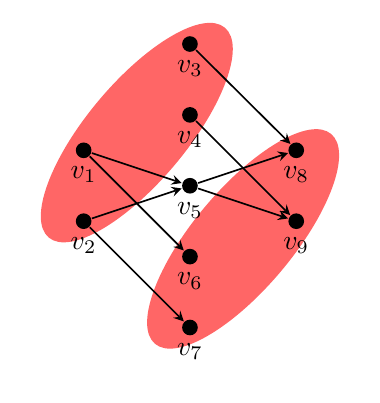
\begin{tikzpicture}[scale=0.9]  
        \draw[rotate around={-40:(0.25,1.75)}, fill=\pathtwocolor, draw=none] (0.25,1.75) ellipse (20pt and 55pt);
        \draw[rotate around={-40:(1.75,0.25)}, fill=\pathtwocolor, draw=none] (1.75,0.25) ellipse (20pt and 55pt);
        
        \node[fill=black, label={[yshift=0.1cm]below:{$v_1$}}] (A1) at (-0.5,1.5) {};
        \node[fill=black, label={[yshift=0.1cm]below:{$v_2$}}] (A2) at (-0.5,0.5) {};
        \node[fill=black, label={[yshift=0.1cm]below:{$v_3$}}] (B1) at (1,3) {};
        \node[fill=black, label={[yshift=0.1cm]below:{$v_4$}}] (B2) at (1,2) {};
        \node[fill=black, label={[yshift=0.1cm]below:{$v_5$}}] (B3) at (1,1) {};
        \node[fill=black, label={[yshift=0.1cm]below:{$v_6$}}] (B4) at (1,0) {};
        \node[fill=black, label={[yshift=0.1cm]below:{$v_7$}}] (B5) at (1,-1) {};
        \node[fill=black, label={[yshift=0.1cm]below:{$v_8$}}] (C1) at (2.5,1.5) {};
        \node[fill=black, label={[yshift=0.1cm]below:{$v_9$}}] (C2) at (2.5,0.5) {};
        \draw[->] (A1) -> (B3);
        \draw[->] (A1) -> (B4);
        \draw[->] (A2) -> (B3);
        \draw[->] (A2) -> (B5);
        \draw[->] (B1) -> (C1);
        \draw[->] (B3) -> (C1);
        \draw[->] (B2) -> (C2);
        \draw[->] (B3) -> (C2);
        \end{tikzpicture}
        \vspace{0cm} % manual hack
        \captionsetup{justification=centering}
        \caption{A DAG $G$, and an MA-$2$ solution $\{v_1,v_2,v_3,v_4\}, \{v_6,v_7,v_8,v_9\}$, in red, covering $\alpha_2 = 8$ vertices.}
        \label{subfig:G}
    \end{subfigure}
    \hfill
    \begin{subfigure}[b]{0.69\linewidth}
        \centering
        % \includegraphics[width=0.7\linewidth]{figures/Gprime}  
        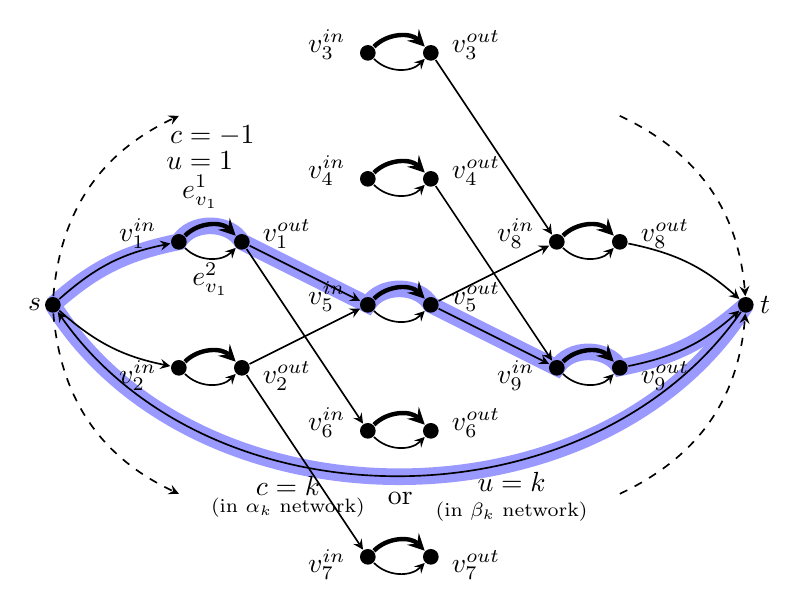
\begin{tikzpicture}[scale=1.6] 

        \useasboundingbox (-2.2,-1.2) rectangle (3.7,3.2);
    
        \node[fill=black, label={[yshift=0.1cm]left:{$v_1^{in}$}}] (A1in) at (-1,1.5) {};
        \node[fill=black, label={[yshift=0.1cm]right:{$v_1^{out}$}}] (A1out) at (-0.5,1.5) {};
    
        \node[fill=black, label={[yshift=-0.1cm]left:{$v_2^{in}$}}] (A2in) at (-1,0.5) {};
        \node[fill=black, label={[yshift=-0.1cm]right:{$v_2^{out}$}}] (A2out) at (-0.5,0.5) {};
    
        \node[fill=black, label={[yshift=0.1cm]left:{$v_3^{in}$}}] (B1in) at (0.5,3) {};
        \node[fill=black, label={[yshift=0.1cm]right:{$v_3^{out}$}}] (B1out) at (1,3) {};
    
        \node[fill=black, label={[yshift=0.1cm]left:{$v_4^{in}$}}] (B2in) at (0.5,2) {};
        \node[fill=black, label={[yshift=0.1cm]right:{$v_4^{out}$}}] (B2out) at (1,2) {};
    
        \node[fill=black, label={[yshift=0.1cm]left:{$v_5^{in}$}}] (B3in) at (0.5,1) {};
        \node[fill=black, label={[yshift=0.1cm]right:{$v_5^{out}$}}] (B3out) at (1,1) {};
    
        \node[fill=black, label={[yshift=0.1cm]left:{$v_6^{in}$}}] (B4in) at (0.5,0) {};
        \node[fill=black, label={[yshift=0.1cm]right:{$v_6^{out}$}}] (B4out) at (1,0) {};    
    
        \node[fill=black, label={[yshift=-0.1cm]left:{$v_7^{in}$}}] (B5in) at (0.5,-1) {};
        \node[fill=black, label={[yshift=-0.1cm]right:{$v_7^{out}$}}] (B5out) at (1,-1) {};
        
        \node[fill=black, label={[yshift=0.1cm]left:{$v_8^{in}$}}] (C1in) at (2,1.5) {};
        \node[fill=black, label={[yshift=0.1cm]right:{$v_8^{out}$}}] (C1out) at (2.5,1.5) {};
    
        \node[fill=black, label={[yshift=-0.1cm]left:{$v_9^{in}$}}] (C2in) at (2,0.5) {};
        \node[fill=black, label={[yshift=-0.1cm]right:{$v_9^{out}$}}] (C2out) at (2.5,0.5) {};
    
        \node[fill=black, label={[xshift=0.1cm]left:{$s$}}] (s) at (-2,1) {};
        \node[fill=black, label={[xshift=-0.1cm]right:{$t$}}] (t) at (3.5,1) {};
    
        \draw[->, ultra thick] (A1in) to [bend left=45] node[midway, yshift=-0.15cm, above]{$\begin{aligned}c&=-1\\[-.2cm] u&=1\\[-.2cm]&e_{v_1}^1\end{aligned}$} (A1out); % top arc
        \draw[->] (A1in) to [bend right=45] node[midway, yshift=0.15cm, below]{$e_{v_1}^2$} (A1out); % bottom arc
        \draw[->, ultra thick] (A2in) to [bend left=45] 
        % node[midway, above, yshift=-0.4cm, xshift=0.1cm]{$\begin{aligned}c&=-1\\[-.2cm] u&=1\end{aligned}$}  
        (A2out); % top arc
        \draw[->] (A2in) to [bend right=45] (A2out); % bottom arc
        \draw[->, ultra thick] (B1in) to [bend left=45]  (B1out); % top arc
        \draw[->] (B1in) to [bend right=45] (B1out); % bottom arc
        \draw[->, ultra thick] (B2in) to [bend left=45]  (B2out); % top arc
        \draw[->] (B2in) to [bend right=45] (B2out); % bottom arc
        \draw[->, ultra thick] (B3in) to [bend left=45]  (B3out); % top arc
        \draw[->] (B3in) to [bend right=45] (B3out); % bottom arc
        \draw[->, ultra thick] (B4in) to [bend left=45]  (B4out); % top arc
        \draw[->] (B4in) to [bend right=45] (B4out); % bottom arc
        \draw[->, ultra thick] (B5in) to [bend left=45]  (B5out); % top arc
        \draw[->] (B5in) to [bend right=45] (B5out); % bottom arc
        \draw[->, ultra thick] (C1in) to [bend left=45] (C1out); % top arc
        \draw[->] (C1in) to [bend right=45] (C1out); % bottom arc
        \draw[->, ultra thick] (C2in) to [bend left=45]  (C2out); % top arc
        \draw[->] (C2in) to [bend right=45] (C2out); % bottom arc
    
        \draw[->] (A1out) -> (B3in);
        \draw[->] (A1out) -> (B4in);
        \draw[->] (A2out) -> (B3in);
        \draw[->] (A2out) -> (B5in);
        \draw[->] (B1out) -> (C1in);
        \draw[->] (B3out) -> (C1in);
        \draw[->] (B2out) -> (C2in);
        \draw[->] (B3out) -> (C2in);
    
        \draw[->, dashed] (s) to [bend left=30] (-1,2.5);
        \draw[->] (s) to [bend left=15] (A1in);
        \draw[->] (s) to [bend right=15] (A2in);
        \draw[->, dashed] (s) to [bend right=30] (-1,-0.5);
    
        \draw[->, dashed] (2.5,2.5) to [bend left=30] (t);
        \draw[->] (C1out) to [bend left=15] (t);
        \draw[->] (C2out) to [bend right=15] (t);
        \draw[->, dashed] (2.5,-0.5) to [bend right=30] (t);
        
        \draw[->] (t) to [bend left=55] node[midway, below, yshift=2.4cm]{$\begin{array}{c}c=k\\[-0.2cm]\scriptsize{\text{(in $\alpha_k$  network)}}\end{array}$ or $\begin{array}{c}u=k\\[-0.1cm]\scriptsize{\text{(in $\beta_k$ network)}}\end{array}$} (s);
    
        \begin{pgfonlayer}{background}
            \draw[-,\pathonecolor, line width=6pt] (s.center) to [bend left=15] (A1in.center) to [bend left=60] (A1out.center) to (B3in.center) to [bend left=60] (B3out.center) to (C2in.center) to [bend left=60] (C2out.center) to [bend right=15] (t.center);
            \draw[-,\pathonecolor, line width=6pt] (t.center) to [bend left=58] (s.center);
        \end{pgfonlayer}
        
        \end{tikzpicture}
        
        \captionsetup{justification=centering}
        \caption{The flow network $G'$ of $G$, and an MPS-$2$ solution $(v_1,v_5,v_9)$, in blue, of $2$-norm equal to $6 + 2 \cdot 1 = 8 = \alpha_2$.}
        \label{subfig:Gprime}
    \end{subfigure}
    \caption{A DAG $G$ and its corresponding $\alpha_k$ and $\beta_k$ networks $G'$, with their difference on edge $(t,s)$ shown. Namely, in the $\alpha_k$ network, the edge $(t,s)$ gets cost $k$, while in the $\beta_k$ network, it gets capacity $k$. For clarity, most edges of the form $(s,v^{in})$ and $(v^{out},t)$ are omitted. The edges of type $e_v^1$ are drawn thicker, and have cost $c=-1$ and capacity $u=1$.}
    \label{fig:reductions}
\end{figure}


\section{Maximum Coverage $k$-antichains in Almost Linear Time}\label{sec:MA-kAlmostLinear}

We first prove how to obtain \Cref{thm:almostLinear} for MPS-$k$ and MCP-$k$.

\begin{lemma}[\Cref{thm:almostLinear}, part I]
    Given a DAG $G = (V, E)$ and a positive integer $k$, we can solve the problems MCP-$k$ and MPS-$k$ in almost optimal $O(|E|^{1+o(1)}+ \texttt{output})$ time.
\end{lemma}
\begin{proof}
    We build the $\alpha_k$ network (see \Cref{sec:preliminaries}) and compute a minimum cost circulation $f$ in $E^{1+o(1)}$ time~\cite{chen2022maximum,van2023deterministic}. Circulation $f$ can be decomposed into a collection of $|f|$ paths $\paths_f$ (for solving MPS-$k$) or $|f|$ disjoint chains $\chains_f$ such that $V(\paths_f) = V(\chains_f)$ (for solving MCP-$k$). By construction (see discussion in \Cref{sec:preliminaries}), the cost of $f$ is $c(f) = -|V(\paths_f)| + k|\paths_f|$, since $f$ minimizes this cost it also minimizes $|V\setminus V(\paths)| + k|\paths|$, and thus $\paths_f$ is a MPS-$k$. We decompose $f$ into $\paths_f$ in $O(|E| + \texttt{output})$ time~\cite{kogan2022beating,caceres2024practical}. We can get $\chains_f$ from $f$ in $O(|E|\log{|f|}) = O(|E|\log{|V|}) = |E|^{1+o(1)}$ time~\cite{caceres2023minimum}. In~\cite[Corollary 6]{caceres2023minimum}, it is additionally stated that $\chains_f$ can be obtained from $\paths_f$ by removing the repeated vertices (up to one copy) from the paths of $\paths_f$. In other words, there is a one-to-one correspondence between $\chains_f$ and $\paths_f$ such that $C \in \chains_f$ is a subsequence of its corresponding $P \in \paths_f$. Next, we note that for every $P\in \paths_f$, $c_P := |P\setminus V(\paths_f \setminus \{P\})| \ge k$; indeed, if $c_P < k$ then the $k$-norm of $\paths_f \setminus \{P\}$ is $k-c_P$ units smaller than the $k$-norm of $\paths_f$, a contradiction. Moreover, since also $V(\chains_f) = V(\paths_f)$, the corresponding $C \in \chains_f$ to $P$ must cover at least those $c_P$ vertices, and thus for every $C \in \chains_f, |C| \ge c_P \ge k$. As such, the $k$-norm of $\chains_f^V$ is exactly the $k$-norm of $\paths_f$, by \Cref{lem:relations}, and thus $\chains_f^V$ is a MCP-$k$.
\end{proof}

Now we prove how to obtain \Cref{thm:almostLinear} for MP-$k$ and MC-$k$.

\begin{lemma}[\Cref{thm:almostLinear}, part II]\label{lem:almostLinear2}
    Given a DAG $G = (V, E)$ and a positive integer $k$, we can solve the problems MP-$k$, MC-$k$ in almost optimal $O(|E|^{1+o(1)}+ \texttt{output})$ time.
\end{lemma}
\begin{proof}
     We build the $\beta_k$ network (see \Cref{sec:preliminaries}) and compute a minimum cost circulation $f$ in $E^{1+o(1)}$ time~\cite{chen2022maximum,van2023deterministic}. Circulation $f$ can be decomposed into a collection of $|f|$ paths $\paths_f$ (for solving MP-$k$) or $|f|$ disjoint chains $\chains_f$ such that $V(\paths_f) = V(\chains_f)$ (for solving MC-$k$). By construction (see discussion in \Cref{sec:preliminaries}), the cost of $f$ is $c(f) = -|V(\paths_f)|$, since $f$ minimizes this cost, $\paths_f$ is a MP-$k$ and $\chains_f$ is a MC-$k$. We decompose $f$ into $\paths_f$ in $O(|E|+\texttt{output})$ time~\cite{kogan2022beating,caceres2024practical} and into $\chains_f$ in $O(|E|\log{|f|}) = O(|E|\log{|V|}) = E^{1+o(1)}$ time~\cite{caceres2023minimum}.
\end{proof}

The proof of \Cref{thm:GKCollections} gives an explicit description of the corresponding antichain collections derived from a minimum cost circulation of the $\alpha_k$ and $\beta_k$ networks. Next, we show how to compute (from the circulation) such antichain collections efficiently. For completeness, in \Cref{appendix:GKProof}, we include a complete proof of \Cref{thm:GKCollections}, adapting the proof of Schrijver to the case of sets (paths and antichains) of vertices.

\begin{lemma}\label{lem:antichainsExtraction}
    Given a minimum cost circulation $f$ of the $\alpha_k$ network (resp. $\beta_k$ network). We can compute a MA-$k$ (resp. a MAS-$k$ and MAP-$k$) in time $|E|^{1+o(1)}$ (deterministic) or in time $\tilde{O}(|E|)$ (Las Vegas w.h.p. and in expectation).
\end{lemma}
\begin{proof}
    Since there are no negative cost cycles in the residual $G'_f$, the function $d: V' \to \ints$ such that $d(v')$ is the distance of a shortest (minimum cost) path from $s$ to $v'$ in $G'_f$, is well defined. In fact, we can compute $d$ in $\tilde{O}(|E|)$ (Las Vegas w.h.p. and in expectation) by using~\cite{bernstein2022negative,bringmann2023negative}. Alternatively, we can compute $d$ in $E^{1+o(1)}$ time via a well-known reduction to minimum cost flow: use the costs of $G'_f$ as the cost of the reduction and add a global sink $t'$ connecting every $v'\in V'$ to $t'$ with an edge with $\ell(v', t) = u(v', t) = 1$, the resulting minimum flow can be decomposed into $|V'|$ shortest paths from $s$. Instead of decomposing the paths, we can obtain $d$ in $O(|E|)$ time with a simple DFS from $s$ following non-$0$ flow edges (see e.g.~\cite{ahuja1993network}). The proof of \Cref{thm:GKCollections} defines $U_i :=  \{v' \in V' \mid d(v') \ge i + d(t)\}$ and $A_i = \{v\in V\mid v^{in} \in U'_i \land v^{out} \not\in U'_i\}$ for every $i\in\{1,\ldots d(s)-d(t)\}$. It is proven that $\antichains_f = \{A_1, \ldots, A_{d(s)-d(t)}\}$ is a collection of antichains and that it is a MA-$k$ in the $\alpha_k$ network and a MAS-$k$ in the $\beta_k$ network. Note that $A_i$ corresponds to the set of vertices $v\in V$ such that $d(v^{in}) \ge i + d(t)$ and $d(v^{out}) < i + d(t)$. In particular, if $d(v^{in}) > d(v^{out})$, then $v \in A_j$ for $j \in \{d(v^{out}) - d(t) + 1, \ldots, d(v^{in})-d(t)\}$. As such, we can build $\antichains_f$ in $O(|E|)$ time by checking each edge $(v^{in}, v^{out})$ and placing $v$ in one such corresponding antichain (e.g. in $A_{d(v^{in})-d(t)}$) when $d(v^{in}) > d(v^{out})$. By \Cref{lem:relations}, $\antichains^V$ is a MAP-$k$.
\end{proof}

We use this lemma to prove the final part of \Cref{thm:almostLinear}.

\begin{lemma}[\Cref{thm:almostLinear}, part III]\label{lem:almostLinear3}
    Given a DAG $G = (V, E)$ and a positive integer $k$, we can solve the problems MA-$k$, MAP-$k$ and MAS-$k$ in almost optimal $O(|E|^{1+o(1)})$ time.
\end{lemma}
\begin{proof}
    Compute a minimum cost circulation $f$ in the $\alpha_k$ network (resp. $\beta_k$ network) in $|E|^{1+o(1)}$ time~\cite{chen2022maximum,van2023deterministic}, and use \Cref{lem:antichainsExtraction} to obtain a MA-$k$ (resp. MAS-$k$ and MAP-$k$).
\end{proof}

\section{Maximum Coverage $k$-antichains in Parameterized Near Linear Time}\label{sec:nearLinear}

The algorithms in \Cref{thm:nearLinear} implement a simple cycle-canceling approach boosted by the recent developments on finding negative cost cycles~\cite{bernstein2022negative,bringmann2023negative}. A well-known result from the theory of network flows~\cite{williamson2019network} states that for a feasible flow $f$, $f$ is a minimum cost circulation iff there is no negative cost cycle\footnote{The cost of a cycle is the sum its edges' costs.} in $G'_f$.  In fact, a negative cost cycle in $G'_f$ can be used to obtain a flow of cost at most $c(f)-1$, deriving the following result

\begin{lemma}\label{lem:cycleCancelingFast}
    Let $c^*$ be the minimum cost of a circulation in a flow network $G', \ell, u, c$. Given a feasible flow $f$, we can compute a minimum cost flow in time $\tilde{O}((c(f)-c^*+1)|E|)$. Algorithm is randomized Las Vegas and running time is with high probability (and in expectation).
\end{lemma}

Note that a feasible circulation $f$ in the $\alpha_k$ and $\beta_k$ networks can be decomposed into $\paths_f$ or $\chains_f$ (see \Cref{sec:preliminaries}). Moreover, in the $\beta_k$ network, $c(f)$ is exactly $-|V(\paths_f)|$,\footnote{Assuming $f(e^1_v) \ge f(e^2_v)$. In other words, there exists another circulation $c(f') = -|V(\paths_f)|$.} and thus the minimum cost of a circulation is $-\beta_k$. Plugging in \Cref{lem:cycleCancelingFast} we obtain.

\begin{lemma}[\Cref{thm:nearLinear}, part II]\label{lem:nearLinear2}
    Given a DAG $G = (V, E)$ and a positive integer $k$, we can solve the problems, MAP-$k$, MAS-$k$, MP-$k$ and MC-$k$ in parameterized near optimal $\tilde{O}(\beta_k|E|)$ time. Algorithms are randomized Las Vegas and running times are with high probability (and in expectation).
\end{lemma}

To extract the MAP-$k$ and MAS-$k$ from the minimum cost circulation we use \Cref{lem:antichainsExtraction}. In contrast, $c(f) = -|V(\paths_f)| + k|\paths_f|$ in the $\alpha_k$ network and its minimum cost $\alpha_k-|V|$. 

We exploit the well-known \emph{greedy} algorithm for \emph{weighted set cover}~\cite{chvatal1979greedy}. In \emph{minimum weight set cover} the input is a collection of sets $\sets$ such that $\bigcup_{S\in\sets} S = V$,\footnote{The reuse of $V$ in the notation is intentional.} and an associated weight function $w: \sets \to \ints_{\ge 0}$, and the task is to find a subcollection $\sets' \subseteq \sets$ covering all elements, that is $V(\sets') = V$, and minimizing its total weight, where $w(\sets') = \sum_{S\in\sets'} w(S)$. The \texttt{greedy} algorithm maintains the set of uncovered elements $U$ and iteratively picks a set $S$ minimizing the ratio $w(S)/|U\cap S|$ until $U = \emptyset$. It is well-known that \texttt{greedy} is a $\ln{|V|}$ approximation~\cite{chvatal1979greedy}. We show that \texttt{greedy} is a $\ln{|V|}$ approximation for MCP-$k$ and MPS-$k$, and that it can be implemented efficiently, a generalization of the result of Mäkinen et al.~\cite[Lemma 2.1]{makinen2019sparse}.

\begin{lemma}\label{lem:generalizedGreedy}
    We can compute a $\ln{|V|}$ approximation of MCP-$k$ and MPS-$k$ in time $O(|E|\alpha_k\log{(|V|)}/k) = \tilde{O}(\alpha_k|E|/k)$.
\end{lemma}
\begin{proof}
    We define the following weighted set cover instance: the sets are the chains of $G$, and for a chain $C$ its weight is $\min{(|C|, k)}$. Note that a feasible solution for this weighted set cover instance is a chain cover (not necessarily partition), and its weight corresponds to its $k$-norm. As such, MCP-$k$'s are optimal solutions to this problem. Moreover, \texttt{greedy} is a $\ln{|V|}$ approximation~\cite{chvatal1979greedy}. We next show how to compute such a greedy solution efficiently. For this, recall that \texttt{greedy} at each step, chooses the chain $C$ minimizing the ratio $w(C)/|U \cap C| = \min{(|C|, k)}/|U \cap C|$, where $U$ is the set of \emph{uncovered} vertices. First, note that there is always a chain $C \subseteq U$ minimizing this ratio, and thus we assume $C \subseteq U$, and the task becomes to find a chain $C \subseteq U$ minimizing the ratio $\min{(|C|, k)}/|C|$. Note that this also ensures that the chain collection found by \texttt{greedy} is a chain partition. Second, if there is no chain $C \subseteq U$ with $|C| > k$, then the ratio is always one and any such chain minimizes the ratio, when \texttt{greedy} reaches this point it can just output every vertex in $U$ in a separated singleton path. Otherwise, \texttt{greedy} must find a chain $C\subseteq U$ minimizing $k/|C|$, but since $k$ is a constant for this minimization, it is equivalent to finding a chain $C \subseteq U$ maximizing $|U|$. Such a chain can be obtained by finding a path covering the most vertices from $U$. Mäkinen et~al.~\cite[Lemma 2.1]{makinen2019sparse} show how to compute such a path in $O(|E|)$ time. Since we stop \texttt{greedy} as soon as there is no chain $C \subseteq U$ with $|C| > k$, the running time of our approach is the number of chains $|C| > k$ times $O(|E|)$. Finally, since each chain $|C| > k$ contributes $k$ to the $k$-norm $O(\alpha_k \log{|V|})$ of the output cover, the number of such chains if $O(\alpha_k \log{|V|}/k)$. Note that the $k$-norm of the set of paths and the chain partition output by \texttt{greedy} is the same, by \Cref{lem:relations}.
\end{proof}

This result suffices to show the first part of \Cref{thm:nearLinear}.


\begin{lemma}[\Cref{thm:nearLinear}, part I]\label{lem:nearLinear1}
    Given a DAG $G = (V, E)$ and a positive integer $k$, we can solve the problems, MCP-$k$, MPS-$k$ and MA-$k$ in parameterized near optimal $\tilde{O}(\alpha_k|E|)$ time. Algorithms are randomized Las Vegas and running times are with high probability (and in expectation).
\end{lemma}
\begin{proof}
 We use \Cref{lem:generalizedGreedy} to compute a collection of paths $\paths$ whose $k$-norm is at most $\alpha_k \ln{|V|}$ in $\tilde{O}(\alpha_k|E|)$ time. These paths correspond to a circulation $f$ in the $\alpha_k$ network. The cost $f$ of this circulation is then $c(f) = -|V(\paths)| + k|\paths| \le \alpha_k\ln{|V|} - |V|$, and since the minimum cost of a circulation is $\alpha_k - |V|$ we can use \Cref{lem:cycleCancelingFast} to obtain a minimum cost circulation in $\tilde{O}(\alpha_k |E|)$ time. As in the proof of \Cref{lem:almostLinear2}, we can obtain a MCP-$k$ and a MPS-$k$ from the minimum cost flow circulation (\texttt{output} size for MPS-$k$ is $O(\alpha_k|E|)$). We use \Cref{lem:antichainsExtraction} to obtain a MA-$k$.
\end{proof}


\section{Approximate Maximum Coverage $k$-antichains using Greedy}\label{sec:approxAlgo}

In the \emph{maximum coverage $k$-sets} version of set cover, the sought solution consists of $k$ sets, covering the maximum number of elements, and in this case \texttt{greedy} is stopped after $k$ iterations. It is well-known that this version of \texttt{greedy} is a $(1-1/e)$ approximation~\cite{hochbaum1996approximating}. When applied to the collection of chains/paths or antichains of a DAG, we automatically obtain the approximation ratio claimed in \Cref{thm:approxAlgo}. Therefore, the main purpose of this section is to provide a fast implementation of \texttt{greedy} in these contexts. 

In a series of works~\cite{felsner2003recognition,kowaluk2008path,makinen2019sparse} it was shown how to efficiently compute \texttt{greedy} chains/paths in $O(|E|)$ time per chain/path, the first part of \Cref{thm:approxAlgo} follows.


\begin{lemma}[\Cref{thm:approxAlgo}, part I]\label{lem:approxAlgo1}
    Given a DAG $G = (V, E)$ and a positive integer $k$, there exist $(1-1/e)$-approximation algorithms solving MP-$k$ and MC-$k$ in $O(k|E|)$ time.
\end{lemma}

We show how to efficiently compute a maximum-sized antichain $A\subseteq U$ for some subset $U\subseteq V$. We adapt a well-known reduction from MPC to minimum flow~\cite{ntafos1979path} to work with minimum path covers only required to cover $U$ instead of the whole $V$.

\begin{lemma}\label{lem:subsetMPC}
    There exists a reduction to minimum flow for the problem of finding a minimum cardinality set of paths covering $U\subseteq V$. Moreover, we can recover a maximum-sized antichain $A\subseteq U$ from a minimum flow in this network in $O(|E|)$ time.
\end{lemma}
\begin{proof}
    For $U = V$, the well-known reduction to minimum flow corresponds to $G'$ as in Schrijver's reduction but without the edge $(t,s)$ and only one copy of edges $(v^{in}, v^{out})$ for $v \in V$ with $\ell(v^{in}, v^{out}) = 1$, all other (non-specified) values for $\ell$ and $u$ are set to default (see \Cref{sec:preliminaries}). Cáceres et~al.~\cite{caceres2022sparsifying,caceres2022minimum} show that a minimum flow $f$ in this network corresponds to a MPC of $G$ (by decomposing $f$) and a maximum-sized antichain can be obtained in $O(|E|)$ time by traversing the residual $G'_f$ from $t$: the maximum-sized antichain corresponds to the vertices $v \in V$ such that $v^{out}$ is reached by $t$ in $G'_f$ but $v^{in}$ is not. Here, we prove that we obtain the same result when only required to cover $U \subseteq V$ by setting $\ell(v^{in}, v^{out}) = 1$ only for $v \in U$. First, note that a flow in this modified network can be decomposed into a collection of paths covering $U$ and a collection of paths covering $U$ corresponds to a feasible flow in this modified network. As such, a minimum flow $f$ in this modified network can be decomposed into a minimum cardinality set of paths covering $U\subseteq V$. Moreover, consider the vertices $V_t$ reached by $t$ in the residual $G'_f$ of this modified network. We define $A \subseteq U$ as $A = \{v \in U \mid v^{out}\in V_t \land v^{in} \not\in V_t\}$. First note that, if (by contradiction) there is a vertex $u \in A$ reaching a vertex $v\in A$ in $G$, then $u^{out}$ reaches $v^{in}$ in $G'$ and also in $G'_f$ (edges have default $\infty$ capacity), a contradiction since $v^{in}\not\in V_t$. As such, $A$ is an antichain. Moreover, by definition, $V_t$ is a $ts$ cut and all edges entering $V_t$ have flow equal to their lower bound. Since there is exactly $|f|$ units of flow entering $V_t$ (by flow conservation), then $|A| = |f|$, and thus $A$ is a maximum-sized antichain $A \subseteq U$. Computing $A$ reduces to computing $V_t$, which can be done in $O(|E|)$ time.
\end{proof}

Therefore, a simple strategy to obtain the $k$ \texttt{greedy} antichains is to solve the minimum flow problem defined in \Cref{lem:subsetMPC} $k$ times. Our final result speeds up this computation by noting that a minimum flow obtained in the $i$-th step of \texttt{greedy} can be used as an initial solution for the $i+1$ step. A well-known result from the theory of network flows~\cite{williamson2019network} states that for a feasible flow $f$, $f$ is a minimum flow if and only if there is not path from $t$ to $s$ in $G'_f$. A $ts$-path in $G'_f$ is known as a \emph{decrementing path} and it can be used to obtain a flow of value at most $|f|-1$. As such, starting from a feasible flow $f$, we can obtain a minimum flow $f^*$ by finding at most $|f|-|f^*|$ decrementing paths in total $O((|f|-|f^*|+1)|E|)$ time.

\begin{lemma}[\Cref{thm:approxAlgo}, part II]\label{lem:approxAlgo2}
    Given a DAG $G = (V, E)$ and a positive integer $k$, there exist $(1-1/e)$-approximation algorithm solving MA-$k$ in time $O(\alpha_1^2|V| + (\alpha_1+k)|E|)$.
\end{lemma}
\begin{proof}
    We compute a MPC in time $O(\alpha_1^2|V| + (\alpha_1+k)|E|)$~\cite{caceres2022sparsifying,caceres2022minimum}, compute the corresponding minimum flow $f_1$ in the reduction of \Cref{lem:subsetMPC} and obtain the first \texttt{greedy} antichain $A_1$ in $O(|E|)$ time. To obtain the $i$-th \texttt{greedy} antichain $A_i$, for $i > 1$, we assume that $U_{i}$ are the vertices still uncovered in iteration $i$, that is $U_{i} = V \setminus \bigcup_{j = 1}^{i-1} A_j$, and that $f_{i-1}$ is a minimum flow as in \Cref{lem:subsetMPC} for $U_{i-1}$. To compute a minimum flow $f_i$ for $U_i$ we use $f_{i-1}$ as an initial solution. Note that $f_{i-1}$ is a feasible flow in the network for $U_{i}$ since $U_{i} \subseteq U_{i-1}$. Obtaining $f_i$ from $f_{i-1}$, can be done by finding $|f_{i-1}| - |f_{i}|$ decrementing $ts$ paths in the corresponding residual networks, each in $O(|E|)$ time. Once we obtain $f_{i}$, we can obtain $A_{i}$ (and $U_{i}$) in $O(|E|)$ time by the second part of \Cref{lem:subsetMPC}. The total running time after computing the MPC is then $O\left(|E|\sum_{i = 2}^k |f_{i-1}| - |f_{i}|+1 \right) = O(|E|(k + |f_1| - |f_k|)) = O((\alpha_1+k)|E|)$.
\end{proof}

Combining the ideas from \Cref{lem:generalizedGreedy,lem:approxAlgo2} we obtain the following approximation algorithm for MAS-$k$ and MAP-$k$.

\begin{lemma}\label{lem:generalizedGreedyAntichains}    
We can compute a $\ln{|V|}$ approximation of MAS-$k$ and MAP-$k$ in $\tilde{O}((\alpha_1+\beta_k/k)|E|)$ time.
\end{lemma}
\begin{proof}
    We start by computing an MPC in $\tilde{O}(\alpha_1|E|)$ time~\cite{makinen2019sparse}, and compute \texttt{greedy} antichains as in the proof of \Cref{lem:approxAlgo2} but stopping the computation whenever the next antichain size is at most $k$ (as we did for chains/paths in the proof of \Cref{lem:generalizedGreedy}) obtaining a collection of greedy antichains: $\antichains$. Note that, following the analysis of \Cref{lem:approxAlgo2}, the running time of computing $\antichains$ is $O((\alpha_1+|\antichains|)|E|)$. We next prove that $\antichains$ is a $\ln{|V|}$ approximation for the MAS-$k$ problem. The bound $|\antichains| \le \beta_k\ln{|V|}/k$ follows by noting that each antichain in $\antichains$ contributes exactly $k$ units to its $k$-norm. The fact that $\antichains$ is a $\ln{|V|}$ approximation follows by noting, as in the proof of \Cref{lem:generalizedGreedy}, that the implementation \texttt{greedy} over the set of antichains of $G$ with weights $\min(|A|,k)$ for antichain $A$, is exactly the first antichains of (unweighted) \texttt{greedy} until their size becomes at most $k$ (for MAS-$k$) plus singleton antichains for the yet uncovered vertices (for MAP-$k$). Both the antichain collection (for MAS-$k$) and antichain partition (for MAP-$k$) have the same $k$-norm by \Cref{lem:relations}.
\end{proof}

\section{Limitations of Greedy on Chains/Paths and Antichains}\label{sec:limitsGreedy}
%% Po, Andreas
%\lowerboundpartition*

\begin{figure}
    \centering
    % \includegraphics[trim={70 400 270 130},clip,scale=.6]{figures/kpath.pdf}
    \begin{subfigure}[b]{\linewidth}
        \centering
        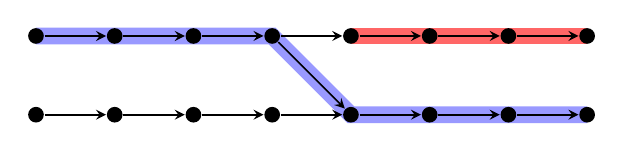
\begin{tikzpicture}
        
            \foreach \i in {1,2,3,4,5,6,7,8} {
                \node[fill=black] (A\i) at (\i-1,1) {};
                \node[fill=black] (B\i) at (\i-1,0) {};
            }
            
            \foreach \i [evaluate=\i as \iplus using int(\i+1)] in {1,2,3,4,5,6,7} {   
                \draw[->] (A\i) -> (A\iplus);
                \draw[->] (B\i) -> (B\iplus);
            }
            \draw[->] (A4) -> (B5);
        
            \begin{pgfonlayer}{background}
                \draw[-,\pathonecolor, line width=6pt] (A1.center) -- (A4.center) -- (B5.center) -- (B8.center);
                \draw[-,\pathtwocolor, line width=6pt] (A5.center) -- (A8.center);
            \end{pgfonlayer}
        
        \end{tikzpicture}
        \captionsetup{justification=centering}
        \caption{The graph $G_2$ from \Cref{lem:upperBoundCoverage-I}}
    \end{subfigure}
    \\[.4cm]
    \begin{subfigure}[b]{\linewidth}
        \centering
        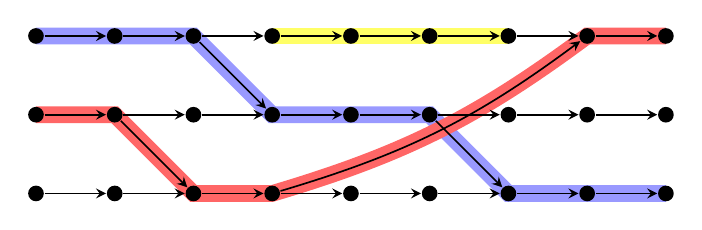
\begin{tikzpicture}
        
            \foreach \i in {1,...,9} {
                \node[fill=black] (A\i) at (\i-1,1) {};
                \node[fill=black] (B\i) at (\i-1,0) {};
                \node[fill=black] (C\i) at (\i-1,-1) {};
            }
            
            \foreach \i [evaluate=\i as \iplus using int(\i+1)] in {1,...,8} {   
                \draw[->] (A\i) -> (A\iplus);
                \draw[->] (B\i) -> (B\iplus);
                \draw[->] (C\i) -> (C\iplus);
            }
            \draw[->] (A3) -> (B4);
            \draw[->] (B2) -> (C3);
            \draw[->] (B6) -> (C7);
            \draw[->] (C4) to[bend right=10] (A8);
        
            \begin{pgfonlayer}{background}
                \draw[-,\pathonecolor, line width=6pt] (A1.center) -- (A3.center) -- (B4.center) -- (B6.center) -- (C7.center) -- (C9.center);
                \draw[-,\pathtwocolor, line width=6pt] (B1.center) -- (B2.center) -- (C3.center) -- (C4.center)  to[bend right=10] (A8.center) -- (A9.center);
                \draw[-,\paththreecolor, line width=6pt] (A4.center) -- (A7.center); 
            \end{pgfonlayer}
        
        \end{tikzpicture}
        \captionsetup{justification=centering}
        \caption{The graph $G_3$ from \Cref{lem:upperBoundCoverage-I}}
    \end{subfigure}
    \caption{Illustrations of the graphs used in \Cref{lem:upperBoundCoverage-I}. The \texttt{greedy} chains are obtained in the order blue, red, yellow.}
    \label{fig:G_2}
\end{figure}

\begin{lemma}[\Cref{thm:upperBoundCoverage}, part I]    
    For every $k\ge 2$, there exists a DAG, such that $k$ \texttt{greedy} chains cover only $3/4$ of $\beta_k$.
    \label{lem:upperBoundCoverage-I}
\end{lemma}
\begin{proof}
    We divide this proof into two parts: first, we give two instances, for $k=2$ and $k=3$, of DAGs such that k \texttt{greedy} chains/paths cover only $3/4$ of $\beta_k$. Secondly, we combine these two instances to create an instance for any $k$. Let $G_2$ be an instance for $k=2$ and $G_3$ be an instance where $k=3$. See \cref{fig:G_2} for $G_2$ and $G_3$. In the $G_2$ instance, $\beta_2$ covers all 16 vertices by selecting both horizontal paths. Greedy, however, covers $8+4 =12$ vertices by selecting the diagonal path first, then only a path of length 4 remains. This gives us the ratio of $12/16=3/4$ for $k=2$. In the $G_3$ instance,  $\beta_3$ covers all 27 vertices by selecting all horizontal paths. \texttt{Greedy}, however, covers $9+6+4=19$ vertices by selecting the blue, red, and yellow chains, in this order.  This gives us the ratio of $19/27 < 3/4$ for $k=3$.

    To obtain the $3/4$ bound for even $k$, we use an instance $\frac{k}{2}\cdot G_2$ ($\frac{k}{2}$ disjoint union of $G_2$). \texttt{Greedy} covers 3/4 portion of vertices of each $G_2$, this gives us the final ratio of $3/4$. For odd $k$, we use an instance $\frac{k-1}{2} \cdot G_2 + 1 \cdot G_3$. \texttt{Greedy} covers at most $3/4$ portion of vertices of $G_3$ and each $G_2$, this gives us the final ratio of $3/4$. 
\end{proof}

\begin{figure}
    \centering
    % \includegraphics[trim={70 400 270 130},clip,scale=.6]{figures/kpath.pdf}
    \begin{subfigure}[b]{\linewidth}
        \centering
        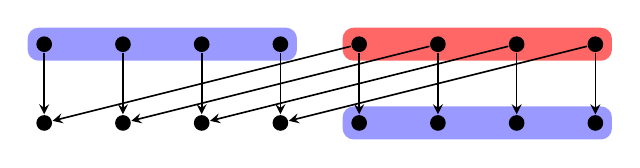
\begin{tikzpicture}
        
            \foreach \i in {1,2,3,4,5,6,7,8} {
                \node[fill=black] (A\i) at (\i-1,1) {};
                \node[fill=black] (B\i) at (\i-1,0) {};
            }
            
            \foreach \i [evaluate=\i as \iplus using int(\i+1)] in {1,...,8} {   
                \draw[->] (A\i) -> (B\i);
            }
            \foreach \i [evaluate=\i as \iplus using int(\i-4)] in {5,...,8} {   
                \draw[->] (A\i) -> (B\iplus);
            }
        
            \begin{pgfonlayer}{background}
                \node[fill=\pathonecolor, draw=none, rectangle, rounded corners, fit=(A1) (A4), inner sep=1mm] (rect) {};
                \node[fill=\pathonecolor, draw=none, rectangle, rounded corners, fit=(B5) (B8), inner sep=1mm] (rect) {};
                \node[fill=\pathtwocolor, draw=none, rectangle, rounded corners, fit=(A5) (A8), inner sep=1mm] (rect) {};
            \end{pgfonlayer}
        
        \end{tikzpicture}
        \captionsetup{justification=centering}
        \caption{The graph $G_2$ from \Cref{lem:upperBoundCoverage-II}}
    \end{subfigure}
    \\[.4cm]
    \begin{subfigure}[b]{\linewidth}
        \centering
        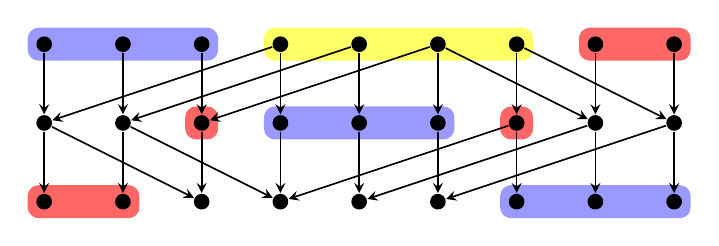
\begin{tikzpicture}
                
            \foreach \i in {1,...,9} {
                \node[fill=black] (A\i) at (\i-1,1) {};
                \node[fill=black] (B\i) at (\i-1,0) {};
                \node[fill=black] (C\i) at (\i-1,-1) {};
            }
            
            \foreach \i [evaluate=\i as \iplus using int(\i+1)] in {1,...,9} {   
                \draw[->] (A\i) -> (B\i);
                \draw[->] (B\i) -> (C\i);
            }
            \draw[->] (A4) -> (B1);
            \draw[->] (A5) -> (B2);
            \draw[->] (A6) -> (B3);
            \draw[->] (A6) -> (B8);
            \draw[->] (A7) -> (B9);
        
            \draw[->] (B1) -> (C3);
            \draw[->] (B2) -> (C4);
            \draw[->] (B7) -> (C4);
            \draw[->] (B8) -> (C5);
            \draw[->] (B9) -> (C6);
        
            \begin{pgfonlayer}{background}
                \node[fill=\pathonecolor, draw=none, rectangle, rounded corners, fit=(A1) (A3), inner sep=1mm] (rect) {};
                \node[fill=\pathonecolor, draw=none, rectangle, rounded corners, fit=(B4) (B6), inner sep=1mm] (rect) {};
                \node[fill=\pathonecolor, draw=none, rectangle, rounded corners, fit=(C7) (C9), inner sep=1mm] (rect) {};
        
                \node[fill=\pathtwocolor, draw=none, rectangle, rounded corners, fit=(C1) (C2), inner sep=1mm] (rect) {};
                \node[fill=\pathtwocolor, draw=none, rectangle, rounded corners, fit=(B3) (B3), inner sep=1mm] (rect) {};
                \node[fill=\pathtwocolor, draw=none, rectangle, rounded corners, fit=(B7) (B7), inner sep=1mm] (rect) {};
                \node[fill=\pathtwocolor, draw=none, rectangle, rounded corners, fit=(A8) (A9), inner sep=1mm] (rect) {};
        
                \node[fill=\paththreecolor, draw=none, rectangle, rounded corners, fit=(A4) (A7), inner sep=1mm] (rect) {};
            \end{pgfonlayer}
        
        \end{tikzpicture}
        \captionsetup{justification=centering}
        \caption{The graph $G_3$ from \Cref{lem:upperBoundCoverage-II}}
    \end{subfigure}
    \caption{Illustrations of the graphs used in \Cref{lem:upperBoundCoverage-II}. The \texttt{greedy} antichains are obtained in the order blue, red, yellow.\label{fig:upperBoundCoverage-II}}
    
\end{figure}

\begin{lemma}[\Cref{thm:upperBoundCoverage}, part II]
    For every $k\ge 2$, there exists a DAG, such that $k$ \texttt{greedy} antichains cover only $3/4$ of $\alpha_k$.
    \label{lem:upperBoundCoverage-II}
\end{lemma}
\begin{proof}
    We divide this proof into two parts: first, we give two instances, for $k=2$ and $k=3$, of DAGs such that $k$ greedy antichains cover only 3/4 of $\alpha_k$. Secondly, we combine these two instances to create an instance for any k. Let $G_2$ be an instance for $k=2$ and $G_3$ be an instance where $k=3$. See \Cref{fig:upperBoundCoverage-II} for $G_2$ and $G_3$. In the $G_2$ instance, $\alpha_2$ covers all 16 vertices by selecting both rows. \texttt{Greedy}, however, covers $8+4 =12$ vertices by selecting the 4 left vertices from the top row and 4 right vertices from the bottom row in the first round, then 4 more vertices in the second round. This gives us the ratio of $12/16=3/4$ for $k=2$. In the $G_3$ instance,  $\alpha_3$ covers all 27 vertices by selecting each of the three rows. \texttt{Greedy}, however, covers $9+6+4=19$ vertices by selecting the blue, red, yellow antichains, in this order. This gives us the ratio of $19/27 < 3/4$ for $k=3$.

    To obtain the 3/4 bound for even $k$, we use $\frac{k}{2}$ copies of $G_2$ (called $G_2^{(1)}, G_2^{(2)}, \dots, G_2^{(\frac{k}{2})}$). Then we add edges from each vertex in $G_2^{(i)}$ to each vertex in $G_2^{(i+1)}$ for all $i$. These edges make sure that no antichain contains vertices from different $G_2^{(i)}$. \texttt{Greedy} covers $3/4$ portion of vertices of each $G_2$, this gives us the final ratio of $3/4$. For odd $k$, we use $\frac{k-1}{2}$ copies of $G_2$  (called $G_2^{(1)}, G_2^{(2)}, \dots, G_2^{(\frac{k-1}{2})}$) and one copy of $G_3$. Then we again add edges from each vertex in $G_2^{(i)}$ to each vertex in $G_2^{(i+1)}$ for all $i$, and also from each vertex in $G_2^{(\frac{k-1}{2})}$ to each vertex in $G_3$. Greedy covers at most $3/4$ portion of vertices of $G_3$ and each $G_2$, this gives us the final ratio of $3/4$. 
\end{proof}

We prove the first part of \Cref{thm:lowerBoundPartition} by providing a class of graphs such that \texttt{greedy} a $\log_4(|V|)$ factor away from the optimal $\alpha_1 = 2$ for the problems MPC and MCP.
We recursively define a class of DAGs $G^C_i$ for $i\geq 2$, each of which can be covered by two paths. %We also attach weights and consider a version of \texttt{greedy} that maximizes the weight of the paths. However, this is just for visual clarity, as we can easily transform the instances to unweighted ones by replacing the vertices with paths of length equal to the weight of the vertex.

\begin{figure}
    \centering
    %\includegraphics[width=0.75\linewidth]{draftImages/lowerBoundGreedyPC.png}

    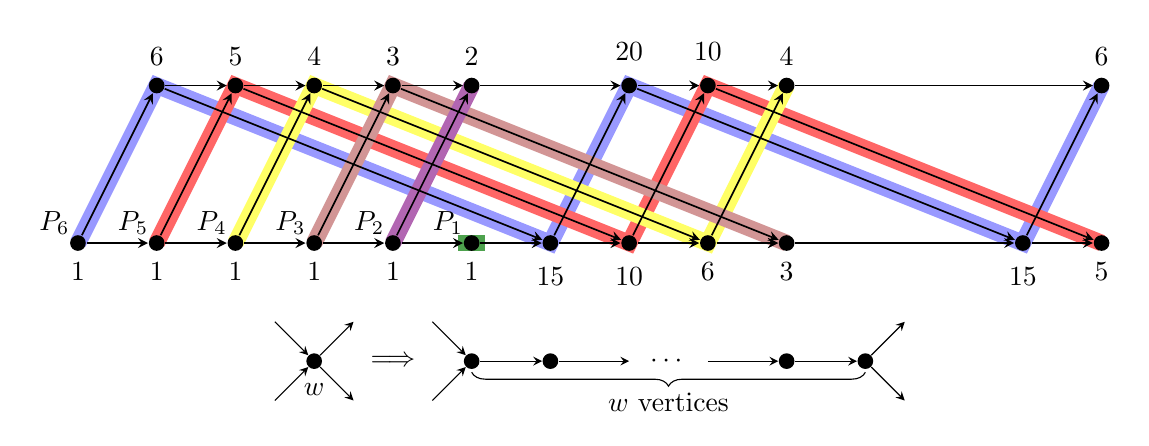
\begin{tikzpicture}[scale=1]
    % 1
    \node[fill=black, label=below:1] (A1) at (0,0) {};
    \node[fill=black, label=above:6] (A2) at (1,2) {};
    \node[fill=black, label=below:15] (A3) at (6,0) {};
    \node[fill=black, label=above:20] (A4) at (7,2) {};
    \node[fill=black, label=below:15] (A5) at (12,0) {};
    \node[fill=black, label=above:6] (A6) at (13,2) {};
    \draw[->] (A1) -> (A2);
    \draw[->] (A2) -> (A3);
    \draw[->] (A3) -> (A4);
    \draw[->] (A4) -> (A5);
    \draw[->] (A5) -> (A6);

    % 2
    \node[fill=black, label=below:1] (B1) at (1,0) {};
    \node[fill=black, label=above:5] (B2) at (2,2) {};
    \node[fill=black, label=below:10] (B3) at (7,0) {};
    \node[fill=black, label=above:10] (B4) at (8,2) {};
    \node[fill=black, label=below:5] (B5) at (13,0) {};
    \draw[->] (B1) -> (B2);
    \draw[->] (B2) -> (B3);
    \draw[->] (B3) -> (B4);
    \draw[->] (B4) -> (B5);

    % 3
    \node[fill=black, label=below:1] (C1) at (2,0) {};
    \node[fill=black, label=above:4] (C2) at (3,2) {};
    \node[fill=black, label=below:6] (C3) at (8,0) {};
    \node[fill=black, label=above:4] (C4) at (9,2) {};
    \draw[->] (C1) -> (C2);
    \draw[->] (C2) -> (C3);
    \draw[->] (C3) -> (C4);

    % 4
    \node[fill=black, label=below:1] (D1) at (3,0) {};
    \node[fill=black, label=above:3] (D2) at (4,2) {};
    \node[fill=black, label=below:3] (D3) at (9,0) {};
    \draw[->] (D1) -> (D2);
    \draw[->] (D2) -> (D3);

    % 5
    \node[fill, label=below:1] (E1) at (4,0) {};
    \node[fill, label=above:2] (E2) at (5,2) {};
    \draw[->] (E1) -> (E2);

    % 6
    \node[fill=black, label=below:1] (F1) at (5,0) {};

    % bottom line
    \draw[->,black] (A1) -> (B1);
    \draw[->,black] (B1) -> (C1);
    \draw[->,black] (C1) -> (D1);
    \draw[->,black] (D1) -> (E1);
    \draw[->,black] (E1) -> (F1);
    \draw[->,black] (F1) -> (A3);
    \draw[->,black] (A3) -> (B3);
    \draw[->,black] (B3) -> (C3);
    \draw[->,black] (C3) -> (D3);
    \draw[->,black] (C3) -> (D3);
    \draw[->,black] (D3) -> (A5);
    \draw[->,black] (A5) -> (B5);

    % top line
    \draw[->,black] (A2) -> (B2);
    \draw[->,black] (B2) -> (C2);
    \draw[->,black] (C2) -> (D2);
    \draw[->,black] (D2) -> (E2);
    \draw[->,black] (E2) -> (A4);
    \draw[->,black] (A4) -> (B4);
    \draw[->,black] (B4) -> (C4);
    \draw[->,black] (C4) -> (A6);

    \node[draw=none] (P6) at (0-0.3,0.55-0.3) {\textcolor{black}{$P_6$}};
    \node[draw=none] (P5) at (1-0.3,0.55-0.3) {\textcolor{black}{$P_5$}};
    \node[draw=none] (P4) at (2-0.3,0.55-0.3) {\textcolor{black}{$P_4$}};
    \node[draw=none] (P3) at (3-0.3,0.55-0.3) {\textcolor{black}{$P_3$}};
    \node[draw=none] (P2) at (4-0.3,0.55-0.3) {\textcolor{black}{$P_2$}};
    \node[draw=none] (P1) at (5-0.3,0.55-0.3) {\textcolor{black}{$P_1$}};

    \begin{pgfonlayer}{background}
        \draw[-,\pathonecolor, line width=6pt] (A1.center) -- (A2.center) -- (A3.center) -- (A4.center) -- (A5.center) -- (A6.center);
        \draw[-,\pathtwocolor, line width=6pt] (B1.center) -- (B2.center) -- (B3.center) -- (B4.center) -- (B5.center);
        \draw[-,\paththreecolor, line width=6pt] (C1.center) -- (C2.center) -- (C3.center) -- (C4.center);
        \draw[-,\pathfourcolor, line width=6pt] (D1.center) -- (D2.center) -- (D3.center);
        \draw[-,\pathfivecolor, line width=6pt] (E1.center) -- (E2.center);
        \draw[-,\pathsixcolor, line width=6pt] (5-0.17,0) -- (5+0.17,0);
    \end{pgfonlayer}

    \begin{scope}[shift={(3,-1.5)}]
        \node[fill=black,label=below:{$w$}] (n) at (0,0) {};
        \draw[->] (-0.5,0.5) to (n);
        \draw[->] (-0.5,-0.5) to (n);
        \draw[->] (n) to (0.5,0.5);
        \draw[->] (n) to (0.5,-0.5);
        \node[fill=none,draw=none] (a) at (1,0) {$\Longrightarrow$};    
        \node[fill=black] (a1) at (2,0) {};
        \node[fill=black] (a2) at (3,0) {};
        \node[fill=black] (a3) at (6,0) {};
        \node[fill=black] (a4) at (7,0) {};
        \draw[->,black] (a1) -> (a2);
        \draw[->,black] (a2) -> (4,0);
        \draw[->,black,draw=none] (a2) to node {$\cdots$} (a3) ;
        \draw[->,black] (5,0) -> (a3);
        \draw[->,black] (a3) -> (a4);
        \draw[->] (1.5,0.5) to (a1);
        \draw[->] (1.5,-0.5) to (a1);
        \draw[->] (a4) to (7.5,0.5);
        \draw[->] (a4) to (7.5,-0.5);

        % Curly brace below the nodes
        \draw [decorate,decoration={brace,amplitude=5pt,mirror,raise=.1em}] (a1.south) -- (a4.south) node[rectangle,midway,yshift=-1.2em]{$w$ vertices};
    \end{scope}

    \end{tikzpicture}
    
    \caption{Illustration of the instance $G^C_6$, with $6$ alternating paths shows as different colors. Each vertex is labeled by its weight $w$ (which can be reduced to $w$ vertices as shown in the bottom of the figure). The green path of a single vertex is $P_1$, and the blue path of length $6$ is $P_6$. The vertices are ordered by $P_6[j-1] \to P_5[j-1] \to \dots \to P_j[j-1]$ for every $j = 1,\dots,6$. Moreover, we ensure that $P_j[j-1] \to P_6[j+1]$ for all $j = 1, \dots, 4=6-2$.}
    \label{fig:lowerBoundGreedyPC}
\end{figure}
%\begin{figure}
%    \centering
%    \includegraphics[width=0.75\linewidth]{figures/greedyPathsWidth2}
%    \caption{Caption}
%    \label{fig:enter-label}
%\end{figure}
See \Cref{fig:lowerBoundGreedyPC} for an illustration of the DAGs $G^C_i = (V^C_i, E^C_i)$. We use \textit{weights $w$} as a shorthand notation for a path of $w$ vertices. Notice that the optimal solution has size 2 by taking top and bottom paths (we call these \textit{straight paths}). We then add paths with vertices that \texttt{greedy} will take (we call these \textit{alternating paths}). The graph $G^C_i$ has $i$ alternating paths $P_1, \dots, P_i$, which always start from the bottom straight path. The number of times that $P_i$ alternates between the top and bottom paths is $i-1$. We use the notation $P_i = \{ P_i[0], \dots, P_i[i] \}$ separated by each alternation.
The base case graph $G^C_1$ consists of one alternating path $P_1$ consisting of a single node with weight $1$. The $i$-th instance $G^C_i$ is constructed by adding the alternating path $P_i$ whose weights $w(P_i[j]) = \binom{i}{j}$.
The vertices of the paths are chosen to respect the following order: $P_i[j-1] \to P_{i-1}[j-1] \to \dots \to P_j[j-1]$ for all $j = 1,\dots,i$ and, in addition, $P_j[j-1] \to P_i[j+1]$ for all $j = 1,\dots,i-2$.
\begin{lemma}[\Cref{thm:lowerBoundPartition}, part I]
    For MPC and MCP, the number of chains/paths taken by \texttt{greedy} on the instances $G^C_i$ is a $\log_4(|V|)$ factor away from the optimal $\alpha_1 = 2$.
\end{lemma}
\begin{proof}
    Note that \texttt{greedy} returns equivalent solutions for both MPC and MCP. 
    We show the following two statements:
    \begin{enumerate}
        \item In $G^C_i$, \texttt{greedy} chooses the alternating path $P_i$ in its first iteration, \label{stm:greedy_path_chooses_largest_path}
        \item $TC(G^C_i) \setminus P_i = TC(G^C_{i-1})$ for all $i > 1$. \label{stm:greedy_path_recurse}
    \end{enumerate}
    The second statement implies that after removing the vertices of $P_i$ from $TC(G^C_i)$\footnote{In the DAG $G$ vertices can be traversed by \texttt{greedy} multiple times in order to reach uncovered vertices, but in the transitive closure $TC(G)$, this is not necessary.}, the set of the remaining edges corresponds to exactly all the paths in $G^C_{i-1}$. As a result, we can recursively use Statement \ref{stm:greedy_path_chooses_largest_path} and \ref{stm:greedy_path_recurse}, to show that the paths $P_i$ are each taken by \texttt{greedy}.

    We first show Statement \ref{stm:greedy_path_chooses_largest_path}. Let $i \geq 2$ and let $Q = \{ Q[0], \dots, Q[|Q|-1] \}$ be the first path chosen by \texttt{greedy}. We will show that $P_i$ is the unique largest weight path in $G^C_i$ and thus, $Q = P_i$. To observe this, we first note that $P_i[0]$ is the unique source node of the DAG, which implies that $Q[0] = P_i[0]$. Assume that $Q \neq P_i$. We will locally change $Q$ until $Q = P_i$ and strictly increase its weight in the process.
    Let $j$ be the smallest index of $Q$ such that $Q[j] \neq P_i[j]$ %(we assume $|Q| \geq j+1$, because otherwise we can just extend $Q$). \andicom{I need to carefully check again if all the indices are correct :)}
    \begin{itemize}
        \item If $j = i-1$ (i.e., $P_i[j]$ is the last vertex of $P_i$), since $P_i$ is the longest alternating path, $|Q| = i$ and $Q[j] = P_{i-1}[j-1]$. We reroute $Q$ to $P_i[j]$, and we have $w(P_{i-1}[j-1]) = \binom{i-1}{j-1} < \binom{i}{j} = w(P_i[j])$.
        \item If $j < i-1$, we reroute $Q$ by passing it through $P_i[j]$, and reconnect it again with a later vertex from $Q$ in the following way:
        \begin{itemize}
            \item If $Q$ passes through $P_i[j+1]$, it did not traverse an alternating edge, and we reroute $Q$ through $P_i[j]$ by using the alternating edge to $P_i[j+1]$. In this case, we replace \[ Q = \{ P_i[0], \dots, P_i[j-1], \mathbf{P_{i-1}[j-1], \dots, P_{j}[j-1]}, P_i[j+1], \dots \} \] by \[ Q = \{ P_i[0], \dots, P_i[j-1], \mathbf{P_i[j]}, P_i[j+1], \dots \}. \] We have \[ w(P_{i-1}[j-1]) + \dots + w(P_{j}[j-1]) = \binom{i-1}{j-1} + \dots + \binom{j}{j-1} < \binom{i}{j} = w(P_i[j]). \]
            \item If $Q$ does not pass through $P_i[j+1]$, we reroute $Q$ through $P_i[j]$ using the unique straight path to reconnect to $Q$. In this case, we replace \[ Q = \{ P_i[0], \dots, P_i[j-1], \mathbf{P_{i-1}[j-1], \dots, P_{i-\ell}[j-1]}, P_{i-\ell}[j], \dots \} \] where $\ell \leq i-j+1$, by \[ Q = \{ P_i[0], \dots, P_i[j-1], \mathbf{P_i[j], P_{i-1}[j], \dots}, P_{i-\ell}[j], \dots \}. \] We have \[ w(P_{i-1}[j-1]) + \dots + w(P_{i-\ell}[j-1]) = \binom{i-1}{j-1} + \dots + \binom{i-\ell}{j-1} < \binom{i}{j} = w(P_i[j]). \]
        \end{itemize}
    \end{itemize}
    We proceed with growing index $j$ until we reach the last vertex of $P_i$. The weight of $Q$ strictly increased after every reroute, and we thus showed that $P_i$ is the unique largest weight path in $G^C_i$. 

    Next, we show Statement \ref{stm:greedy_path_recurse}. Clearly, $TC(G^C_{i-1}) \subseteq TC(G^C_i) \setminus P_i$. To show the opposite inclusion, let $u,v \in V^C_{i-1}$, such that the edge $(u,v)$ is in $TC(G^C_i) \setminus P_i$. Let $u = P_j[\ell]$ and $v = P_k[\ell']$, where $j,k \leq i-1$. We show that there exists a $uv$-path in $G^C_{i-1}$, which shows that the edge $(u,v)$ is also in $TC(G^C_{i-1})$.
    Assume that $u$ and $v$ are covered by different straight paths (otherwise, the straight path is the $uv$-path we are looking for). Then we can consider either $u' = P_j[\ell+1]$ if $j > \ell+1$, or $u' = P_{i-1}[\ell+3]$ if $j = \ell+1$. %In both cases, $u'$ and $v$ are covered by the same straight path, and $\ell+1 \leq \ell'$ if $|P_j| > \ell+1$ or $\ell+3 \leq \ell'$ if $|P_j| = \ell+1$.
    In both cases, $u'$ is the left most vertex on the same straight path as $v$ satisfying that $(u,u')$ is an edge in $TC(G^C_{i-1})$. Thus, also $(u', v)$ is an edge in $TC(G^C_{i-1})$.

    In the unweighted version of $G^C_i$, the number of vertices is the sum of all the weights. That is, $w(V^C_i) = \sum_{j = 1}^i w(P_j)=\sum_{j = 1}^i 2^{j}-1 < 2^{i+1}$, which implies that the number of \texttt{greedy} paths is $i \geq \log_2(|V^C_i|)$. Dividing by $\alpha_1 = 2$, we obtain $\log_4(|V^C_i|)$ for the factor.
\end{proof}

    \begin{figure}[t]
        \centering
    %     \includegraphics[width=0.75\linewidth]{draftImages/lowerBoundGreedyAC.png}
    %     \caption{Caption}
    %     \label{fig:lowerBoundGreedyAC}
    % \end{figure}
    % \begin{figure}
    %     \centering
        % \includegraphics[width=0.5\linewidth]{figures/greedyAntichainsHeight2}
        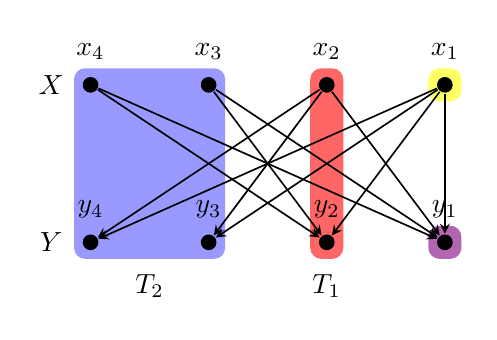
\begin{tikzpicture}[scale=1]       

        % % Add a rounded corner rectangle
        % \draw[fill=\pathonecolor, rounded corners=8pt, draw=none] (1.2, -0.3) rectangle node[rectangle,above,yshift=-2cm] {$T_2$} (3.3, 2.3);
        
        % \draw[fill=\pathtwocolor, rounded corners=8pt, draw=none] (4.2, -0.3) rectangle node[rectangle,above,yshift=-2cm] {$T_1$} (4.8, 2.3);
        % \draw[fill=\paththreecolor, rounded corners=8pt, draw=none] (5.7, -0.3) rectangle (6.3, 0.3);
        % \draw[fill=\pathfivecolor, rounded corners=8pt, draw=none] (5.7, 1.7) rectangle (6.3, 2.3);
    
        \foreach \i [evaluate=\i as \ieval using 4-\i+1] in {1,2,3,4} {
            \node[fill=black,label=above:{$x_{\pgfmathtruncatemacro{\yet}{\ieval}\yet}$}] (A\i) at (1.5*\i,2) {};
            \node[fill=black,label=above:{$y_{\pgfmathtruncatemacro{\yet}{\ieval}\yet}$}] (B\i) at (1.5*\i,0) {};
        }
        \foreach \i in {1,2} {
            \draw[->] (A\i) -> (B3);
            \draw[->] (A\i) -> (B4);
            \draw[->] (A3) -> (B\i);
            \draw[->] (A4) -> (B\i);
        }
        \draw[->] (A3) -> (B4);
        \draw[->] (A4) -> (B3);
        \draw[->] (A4) -> (B4);

        \node[fill=none,draw=none] (A) at (1,2) {$X$};
        \node[fill=none,draw=none] (B) at (1,0) {$Y$};

        \begin{pgfonlayer}{background}
            \node[fill=\pathonecolor, draw=none, rectangle, rounded corners, fit=(A1) (B2), inner sep=1mm, label=below:$T_2$] (rect) {};
    
            \node[fill=\pathtwocolor, draw=none, rectangle, rounded corners, fit=(A3) (B3), inner sep=1mm, label=below:$T_1$] (rect) {};
    
            \node[fill=\paththreecolor, draw=none, rectangle, rounded corners, fit=(A4) (A4), inner sep=1mm] (rect) {};

            \node[fill=\pathfivecolor, draw=none, rectangle, rounded corners, fit=(B4) (B4), inner sep=1mm] (rect) {};
        \end{pgfonlayer}
    
        \end{tikzpicture}
        \caption{Illustration of the graph $G^A_2$ from \Cref{lem:lowerBoundPartition-partII}.}
        \label{fig:lowerBoundGreedyAC}
    \end{figure}


\begin{lemma}[\Cref{thm:lowerBoundPartition}, part II]
    For MAP, there exists a class of DAGs of increasing size, such that the number of antichains taken by \texttt{greedy} is a $\log_4(|V|)$ factor away from the optimal $\beta_1 = 2$.
    \label{lem:lowerBoundPartition-partII}
\end{lemma}
\begin{proof}
    We construct a class of instances $G^A_i = (V^A_i, E^A_i)$ such that $|V^A_i| = 2 \cdot 2^i$, $\beta_1 = 2$ and \texttt{greedy} takes $i+2$ antichains. This implies the factor of $(i+2) / 2 \geq \log_4(|V^A_i|)$. See \Cref{fig:lowerBoundGreedyAC} for an illustration. The undirected graph underlying the DAG $G^A_i$ is bipartite, with $V^A_i = X \cup Y$, $X = \{ x_1, \dots, x_{2^i} \}$ and $Y = \{ y_1, \dots, y_{2^i} \}$. Since the graph is bipartite, $X$ and $Y$ are both antichains that correspond to the optimal solution. We add edges from $X$ to $Y$, such that the following sets become antichains for $1 \leq k \leq i$: $T_k = \{ x_j, y_j \mid 2^{k-1} < j \leq 2^k \}$. We let $(x_j, y_{j'}) \in E^A_i$ if and only if they are not both in the same set $T_k$ (i.e., $|T_k \cap \{ x_j, y_{j'} \}| \leq 1$ for all $1 \leq k \leq i$). Note that if a non-singleton set $U \subseteq V^A_i$ is an antichain, then it is a subset of some $T_k$, $X$ or $Y$. It can easily be verified by induction that \texttt{greedy} chooses the sets $T_k$, from $k=i$ to $1$, with two singleton vertices $x_1$ and $y_1$ left over, that are chosen as two new antichains, hence $i+2$ antichains in total.
\end{proof}



\bibliography{references}

\appendix

\newpage
\section{Overview of problem statements, acronyms and complexity bounds}\label{appendix:acronyms}

In \Cref{tab:acronyms} we recall brief definitions of the problems and symbols from this paper and their state-of-the-art complexity bounds, while in \Cref{tab:our-results} we give an overview of our results.

\begin{table}[h!]
    \newcolumntype{L}[1]{>{\raggedright\arraybackslash}p{#1}}
    \caption{Main acronyms and symbols, and known running times, on input $G = (V,E), k$.}
    \centering
    \begin{tabular}{L{1.1cm}L{7.7cm}L{3.9cm}}
         Symbol     & Meaning & State-of-the-art algorithms \\\Xhline{3\arrayrulewidth}
         MA-$k$; $\alpha_k$     & Maximum Coverage $k$-antichains, i.e.~a set of $k$ antichains whose union size $\alpha_k$ is maximized  & $O(|V|^3)$~\cite{gavril1987algorithms}\newline $(k|E|)^{1+o(1)}$~\cite{kogan2024algorithmic}\newline$|E|^{1+o(1)}$ $1/2$-approx.~\cite{kogan2024algorithmic} \\\hline
         MC-$k$; $\beta_k$     & Maximum Coverage $k$-chains, i.e.~a set of chains whose union size $\beta_k$ is maximized  & $|E|^{1+o(1)}$~\cite{kogan2022beating,caceres2023minimum}\newline Polylog flow calls. \\\hline
         MP-$k$; $\beta_k$     & Maximum Coverage $k$-paths, i.e., a set of $k$ paths whose union size $\beta_k$ is maximized  & $O(|E|^{1+o(1)}+\texttt{output})$~\cite{kogan2022beating}\newline Polylog flow calls.\\\Xhline{3\arrayrulewidth}
         MAP        & A partition of $V$ into the minimum number of antichains, which equals $\beta_1$, the \emph{height} of $G$, by Mirsky's theorem~\cite{mirsky1971dual}  & $O(|E|)$~\cite{mirsky1971dual}\\\hline
         MCP        & A partition of $V$ into the minimum number of chains, which equals $\alpha_1$, the \emph{width} of $G$, by Dilworth's theorem~\cite{dilworth1987decomposition}  & $|E|^{1+o(1)}$~\cite{caceres2023minimum} \newline $O(\alpha_1^2|V|+|E|)$~\cite{caceres2022sparsifying,caceres2022minimum} $\tilde{O}(\alpha_1|E|)$~\cite{makinen2019sparse}\\\hline
         MPC        & A set of paths covering $V$ of minimum cardinality, which is equal to $\alpha_1$ by Dilworth's theorem~\cite{ntafos1979path}  & Same as for MCP $+O(\texttt{output})$~\cite{kogan2022beating} \\\Xhline{3\arrayrulewidth}
         MAP-$k$    & An antichain partition $\antichains$ of minimum $k$-norm $\sum_{A \in \antichains} \min(|A|, k)$, equaling $\beta_k$ by Greene-Kleitman theorems~\cite{greene1976structure,greene1976some}; MAP-$1$=MAP  & No algorithmic result for $k>1$\\\hline
         MCP-$k$    & A chain partition $\chains$ of minimum $k$-norm $\sum_{C \in \chains} \min(|C|, k)$, equaling $\alpha_k$ by Greene-Kleitman theorems~\cite{greene1976structure,greene1976some}; MCP-$1$=MCP  & $|E|^{1+o(1)}$~\cite{kogan2022beating,caceres2023minimum}\newline Polylog flow calls.\\\Xhline{2\arrayrulewidth}
         MAS-$k$    & A set $\antichains$ of antichains of minimum $k$-norm $|V\setminus V(\antichains)| + k|\antichains|$, equaling $\beta_k$ by Greene-Kleitman theorems~\cite{schrijver2003combinatorial}; MAS-$k$ equivalent to MAP-$k$  &  No algorithmic result for $k>1$\\\hline
         MPS-$k$    & A set $\paths$ of paths of minimum $k$-norm $|V\setminus V(\paths)| + k|\paths|$, equaling $\alpha_k$ by Greene-Kleitman theorems~\cite{schrijver2003combinatorial}; MPS-$1$ equivalent to MPC  &  No algorithmic result for $k>1$\\\Xhline{3\arrayrulewidth}
    \end{tabular} 
    \label{tab:acronyms}
\end{table}


\begin{table}[h!]
    \centering
    \caption{Summary of the algorithmic results from this paper, $O(\texttt{output})$ time not shown. \Cref{thm:almostLinear} does a $O(1)$ number of calls to flow solvers, results of \Cref{thm:nearLinear} are randomized, results of \Cref{thm:approxAlgo} are $(1-1/e)$ approximations and results of \Cref{lem:generalizedGreedy,lem:generalizedGreedyAntichains} are $\ln{|V|}$ approximations \label{tab:our-results}}

    \begin{tabular}{lllll}
         Problem&  \Cref{thm:almostLinear} & \Cref{thm:nearLinear}& \Cref{thm:approxAlgo} & \Cref{lem:generalizedGreedy,lem:generalizedGreedyAntichains} \\\Xhline{3\arrayrulewidth}
         MA-$k$&  $|E|^{1+o(1)}$&  $\tilde{O}(\alpha_k|E|)$& $O(\alpha_1^2|V| + (\alpha_1+k)|E|)$ &\\\hline
         MC-$k$, MP-$k$& $|E|^{1+o(1)}$ &  $\tilde{O}(\beta_k|E|)$& $O(k|E|)$&\\\hline
         MAP-$k$, MAS-$k$& $|E|^{1+o(1)}$ &  $\tilde{O}(\beta_k|E|)$& &$\tilde{O}((\alpha_1+\beta_k/k)|E|)$\\\hline
         MCP-$k$, MPS-$k$& $|E|^{1+o(1)}$ &  $\tilde{O}(\alpha_k|E|)$& & $\tilde{O}(\alpha_k|E|/k)$\\\Xhline{3\arrayrulewidth}
    \end{tabular}
    
    
\end{table}

\section{Proof of the Greene-Kleitman Theorems}\label{appendix:GKProof}

\GKCollections*
\begin{proof}
This proof mimics the proofs of ~\cite[Theorem 14.8 \& Theorem 14.10]{schrijver2003combinatorial} for the case of paths/antichains of vertices. We first prove the inequality $\le$, which holds for any $k$ antichains/$k$ paths and any path/antichain collection. For the $\alpha_k$ version, let $\antichains$ be $k$ antichains, $|\antichains| = k$, and $\paths$ a collection of paths. Then, note that 
\begin{align*}
    |V(\antichains)|    &\le |V\setminus V(\paths)| + |V(\paths) \cap V(\antichains)| \\
        &\le |V\setminus V(\paths)| + \sum_{P\in \paths} \sum_{A\in\antichains}|P \cap A| \\
        &\le |V\setminus V(\paths)| + k|\paths|
\end{align*}
where the last inequality follows since a path and an antichain can intersect in at most one vertex, i.e., $|P\cap A| \le 1$. The $\beta_k$ version of the inequality follows by the same argument (by exchanging the roles of $\paths$ and $\antichains$). To prove that the values meet in the optimum we use the $\alpha_k$ and $\beta_k$ networks described in \Cref{sec:preliminaries}. Consider a minimum cost circulation $f$ in one of the networks. As argued in the main paper, if $f$ is minimum in the $\alpha_k$ network, then we can obtain a MPS-$k$ $\paths_f$ by decomposing $f$, and if $f$ is minimum in the $\beta_k$ network, then we can obtain a MP-$k$ $\paths_f$ by decomposing $f$. In both networks, consider the function $d: V' \rightarrow \ints$ such that $d(v')$ is the distance of a shortest (minimum cost) path from $s$ to $v'$ in the residual $G'_f$. First, note that since $f$ is minimum, there are not negative cost cycles in $G'_f$ and thus $d$ is well defined. Moreover, $d(s) = 0$ by definition, and $d(v') \le 0$ for all $v'\in V'$ since there is always a path $P = s, v^{in}, v^{out}, t$ (using $e_v^2$) in $G'_f$ such that all edge costs are $0$ and $v' \in P$. Furthermore, since $d$ is the shortest path distance from $s$ in $G'_f$, it follows that for all $e' = (u', v') \in E'_f$, $d(v') \le d(u') + c(e')$. In particular, if both an edge $e' = (u', v')$ and its reverse are in $E'_f$, then $d(v') = d(u') + c(e')$. For our networks, this implies:

\begin{enumerate}
    \item $d(v') \le d(u')$ if $e' = (u', v') \in E'\setminus (\{e^1_v \mid v \in V\}\cup \{(t,s)\})$, and $d(v') = d(u')$ if $f(e') \ge 1$.
    \par Cost in such edges is $c(e') = 0$ and its reverse is in $E'_f$ if and only if $f(e') \ge 1$.
    \item $d(v^{out}) \le d(v^{in}) - 1$ if $f(e^1_v) = 0$, and $d(v^{out}) \ge d(v^{in}) - 1$ if $f(e^1_v) = 1$.
    \par Cost in such edges is $c(e^1_v) = -1$ and $e^1_v \in E'_f \Leftrightarrow f(e^1_v) = 0 \Leftrightarrow$ reverse of $e^1_v \not\in E'_f$.
    \item For the $\alpha_k$ network, $d(s) = d(t) + k$, since we assume $f(t, s) \ge 1$: otherwise, there is no path of length more than $k$ (one such path would reduce $c(f)$) and by Mirsky's theorem~\cite{mirsky1971dual} a MAP is a MA-$k$ whose coverage ($\alpha_k = |V|$) matches the $k$-norm of $\paths_f = \emptyset$.
    \item For the $\beta_k$ network, we assume $f(t,s) = k$: otherwise we can redefine $f$ to be a different minimum cost circulation with the same cost and $f(t,s) = k$ (e.g. pick arbitrary $v\in V$ and push $k-f(t,s)$ units of flow on $(s, v^{in}), e^2_v, (v^{out}, t)$ and $(t,s)$ at total cost $0$).
\end{enumerate}

We define the following subset of vertices $U_i := \{v' \in V' \mid d(v') \ge i + d(t)\}$ for $i \in \{1, \ldots, d(s) - d(t)\}$. By definition, $U'_i$ is an $st$-cut ($s\in U'_i$, $t\not\in U'_i$). Moreover, there are no edges, other than $(t,s)$ going into $U'_i$ in $G'$: indeed, if $(u', v') \in E'\setminus \{(t,s)\}, u' \not\in U'_i, v'\in U'_i$, then by \textbf{1.} and \textbf{2.}, $d(v') \le d(u')$, but also $d(u') < i + d(t)$ and $d(v') \ge i + d(t)$ implying $d(u') < d(v')$, a contradiction. We use $U_i$ to define subsets of vertices of the input DAG $G$, $A_i = \{v\in V\mid v^{in} \in U'_i \land v^{out} \not\in U'_i\}$. In fact, $A_i$ is an antichain: if $u\neq v \in A$ are such that there is a $uv$ path in $G$, then there is a $u^{out}v^{in}$ path in $G'\setminus \{(t,s)\}$, but such a path would cross from $V'\setminus U_i$ to $U_i$, a contradiction. We define $\antichains_f = \{A_{1}, \ldots, A_{d(s)-d(t)}\}$ to be the collection of antichains extracted from $f$. Note that in the $\alpha_k$ network, by \textbf{3.}, $|\antichains_f| = k$. And in the $\beta_k$ network, by \textbf{4.}, $|\paths_f| = k$. These collections satisfy:

\begin{enumerate}[a.]
    \item $V\setminus V(\paths_f) \subseteq V(\antichains_f)$: indeed, if $v \in V\setminus V(\paths_f)$, then $f(e^1_v) = 0$ and, by \textbf{2.}, $d(v^{out}) \le d(v^{in}) - 1$. But then, $v \in A_{d(v^{in}) - d(t)} \subseteq V(\antichains_f)$. Note that, $1 \le d(v^{out}) + 1 - d(t) \le d(v^{in}) - d(t) \le d(s) - d(t)$ since both $(s, v^{in}), (v^{out}, t) \in E'_f$.
    \item Thus also $V\setminus V(\antichains_f) \subseteq V(\paths_f)$.
\end{enumerate}

For the $\alpha_k$ network we have:
\begin{align*}
    k|\paths_f| &=\\
   \text{(by \textbf{3.})}  &= (d(s) - d(t))f(t,s)\\
  \text{($f$ is circulation)}  &= \sum_{e'=(u',v')\in E'\setminus\{(t,s)\}} (d(u')-d(v'))f(e')\\
    &= \sum_{e'=(u',v')\in E'\setminus (\{e^1_v \mid v \in V\}\cup \{(t,s)\})\})} (d(u')-d(v'))f(e') \\
    &+ \sum_{e^1_v, v \in V} (d(v^{in})-d(v^{out}))f(e^1_v)\\
  \text{(by \textbf{1.})}  &= \sum_{e^1_v, v \in V} (d(v^{in})-d(v^{out}))f(e^1_v) \\
  \text{(by \textbf{2.})}& = |\{v \in V \mid f(e^1_v) = 1 \land d(v^{in})-d(v^{out}) = 1\}|   \\
  &\le |V(\paths_f) \cap V(\antichains_f)|
\end{align*}

For the $\beta_k$ network we have:
\begin{align*}
    k|\antichains_f| &=\\
    \text{(by \textbf{4.})} &= f(t,s) (d(s) - d(t)) \\
    \text{(previous derivation)}&\le   |V(\paths_f) \cap V(\antichains_f)|
\end{align*}


For $\alpha_k$ the proof concludes by:
\begin{align*}
    |V\setminus V(\paths_f)| + k |\paths_f| &=\\
    \text{(by \textbf{a.})} &= |V(\antichains_f)\setminus V(\paths_f)| + k |\paths_f| \\
    \text{(derivation for $\alpha_k$ network)} &\le |V(\antichains_f)\setminus V(\paths_f)| + |V(\paths_f) \cap V(\antichains_f)| \\
    &= |V(\antichains_f)|
\end{align*}

Analogously for $\beta_k$:
\begin{align*}
    |V\setminus V(\antichains_f)| + k |\antichains_f| &=\\
    \text{(by \textbf{b.})} &= |V(\paths_f)\setminus V(\antichains_f)| + k |\antichains_f| \\
    \text{(derivation for $\beta_k$ network)} &\le |V(\paths_f)\setminus V(\antichains_f)| + |V(\paths_f)\cap V(\antichains_f)| \\
    &= |V(\paths_f)|
\end{align*}
\end{proof}

\end{document}